% Appendix Template

\chapter{Tables and Figures} \label{ch:TablesAndFigures}

\section{Test theories and ATA}

\begin{table}[H]
	
	\caption{Example of item bank. \label{tab:bankex}}
	\resizebox{\textwidth}{!}{
		\begin{tabular}{llllllccccccc}
			\toprule
			i & \textsl{ID} & $b$ & $b_{se}$ & \textsl{ES} & \textsl{FORMAT} & \textsl{PROCESS} & \textsl{DOMAIN} & ITEM & ITEM & ENEMY & ENEMY & ENEMY \\
			& & & & & & & & SET 1 &  SET 2 & SET 1 & SET 2 & SET 3\\ 
			\midrule
			1 & M02KL & -2.0 & 1.02 & 0.6& Matching & Problem & Numbers& 1 & 0 & 1 & 0 & 0 \\
			& &  &  & & & solving & &  &  &  &  &  \\
			2 & M35KL & -1.5 & 0.12 & 0.3& Multiple-choice & Knowing & Space & 1& 0& 1 & 0 & 0 \\
			& & & & & & &  and figures & & &  &  & \\
			$\vdots$ & $\vdots$ & $\vdots$ & $\vdots$ & $\vdots$ & $\vdots$ & $\vdots$ & $\vdots$ & $\vdots$ & $\vdots$ & $\vdots$ & $\vdots$ & $\vdots$ \\
			$I-2$ & M03PF & 1.2 & 0.05 & 0.4 & Open-ended & Knowing & Numbers & 0& 1& 1 & 0 & 1 \\
			$I-1$ & M08PF & 0.06 & 0.98 & 0.35 & Multiple-choice & Knowing & Numbers & 0& 1& 1 & 0 & 1 \\
			$I$ & M10ML & 0.75 & 0.4 & 0.12 & Multiple-choice & Knowing & Space & 0 & 0 & 1 & 0 & 1\\
			& & & & & & & and figures &  & & \\
			\bottomrule
	\end{tabular}}
	
\end{table}

\pagebreak

\begin{figure}[H] 
	\centering
	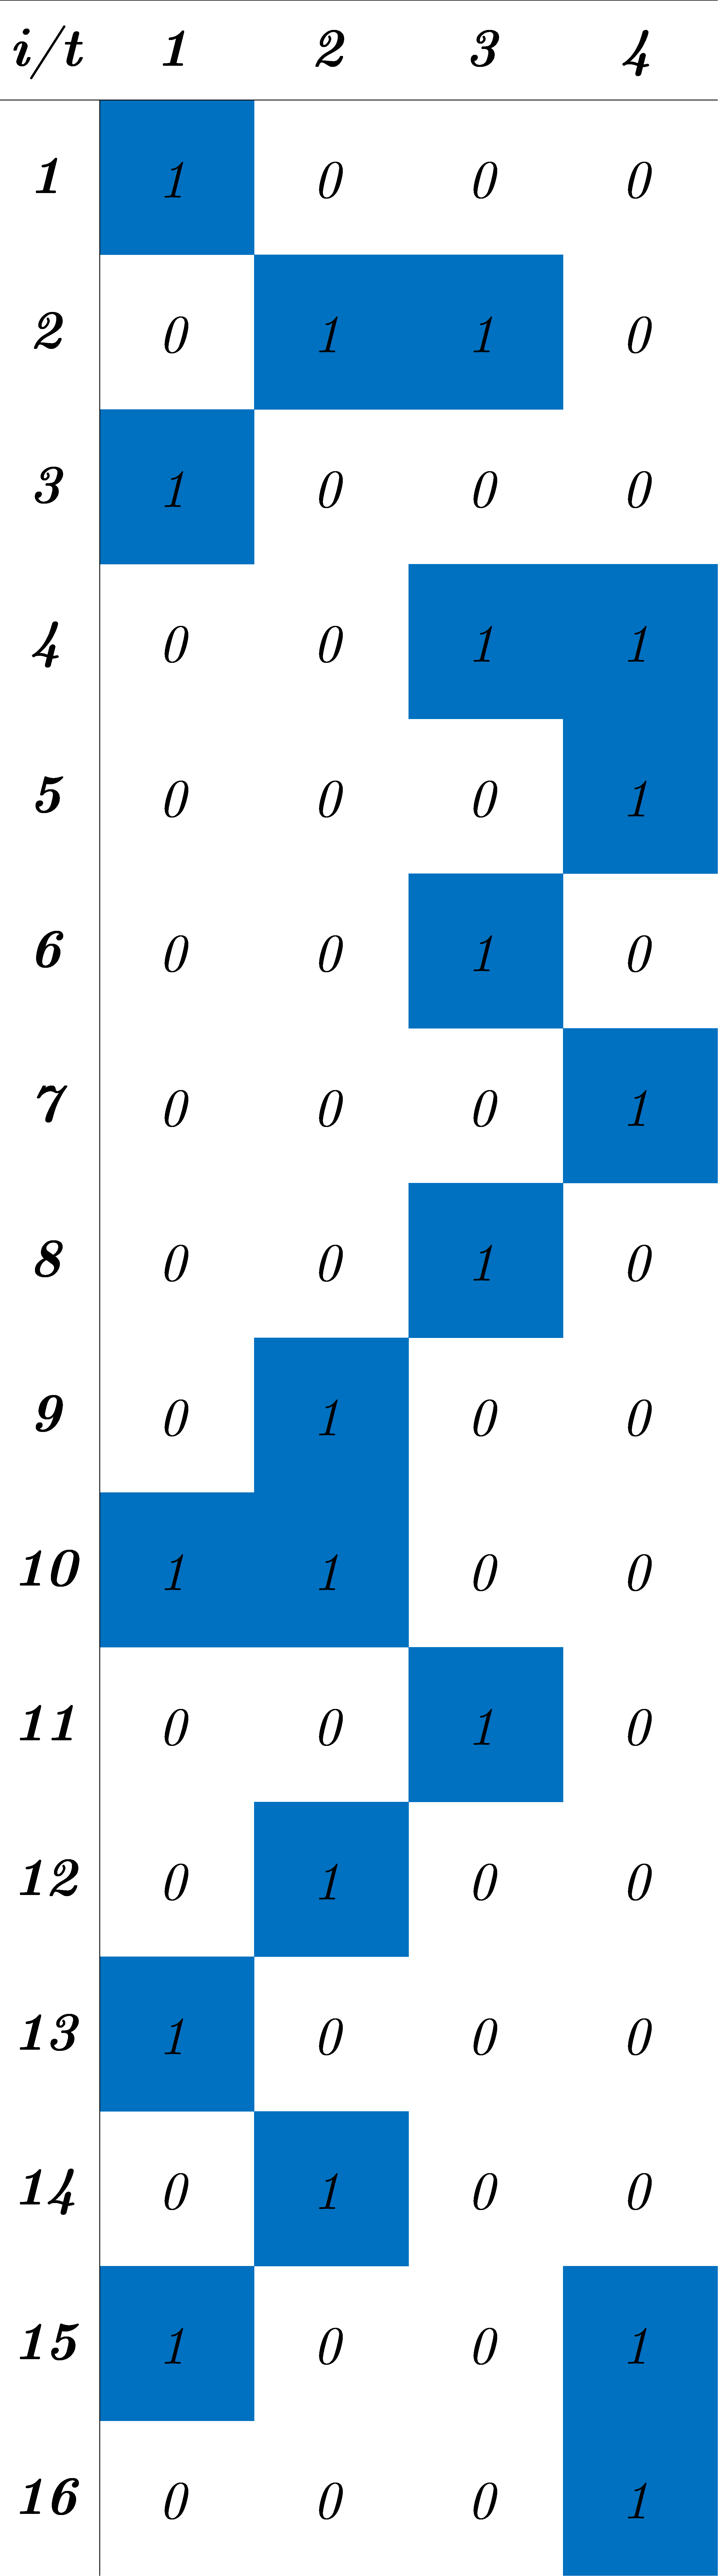
\includegraphics[width=5cm]{Figures/itemsxtests.png}
	\caption{An example of unbalanced \emph{items $\times$ tests} design, for $T=4$ tests with lenght equal to 5 and 2 anchor items (overlap), and $I=16$ items from the pool.}
	\label{fig:itemsxtests}
\end{figure}
\pagebreak

\begin{figure}[H] 
	\centering
	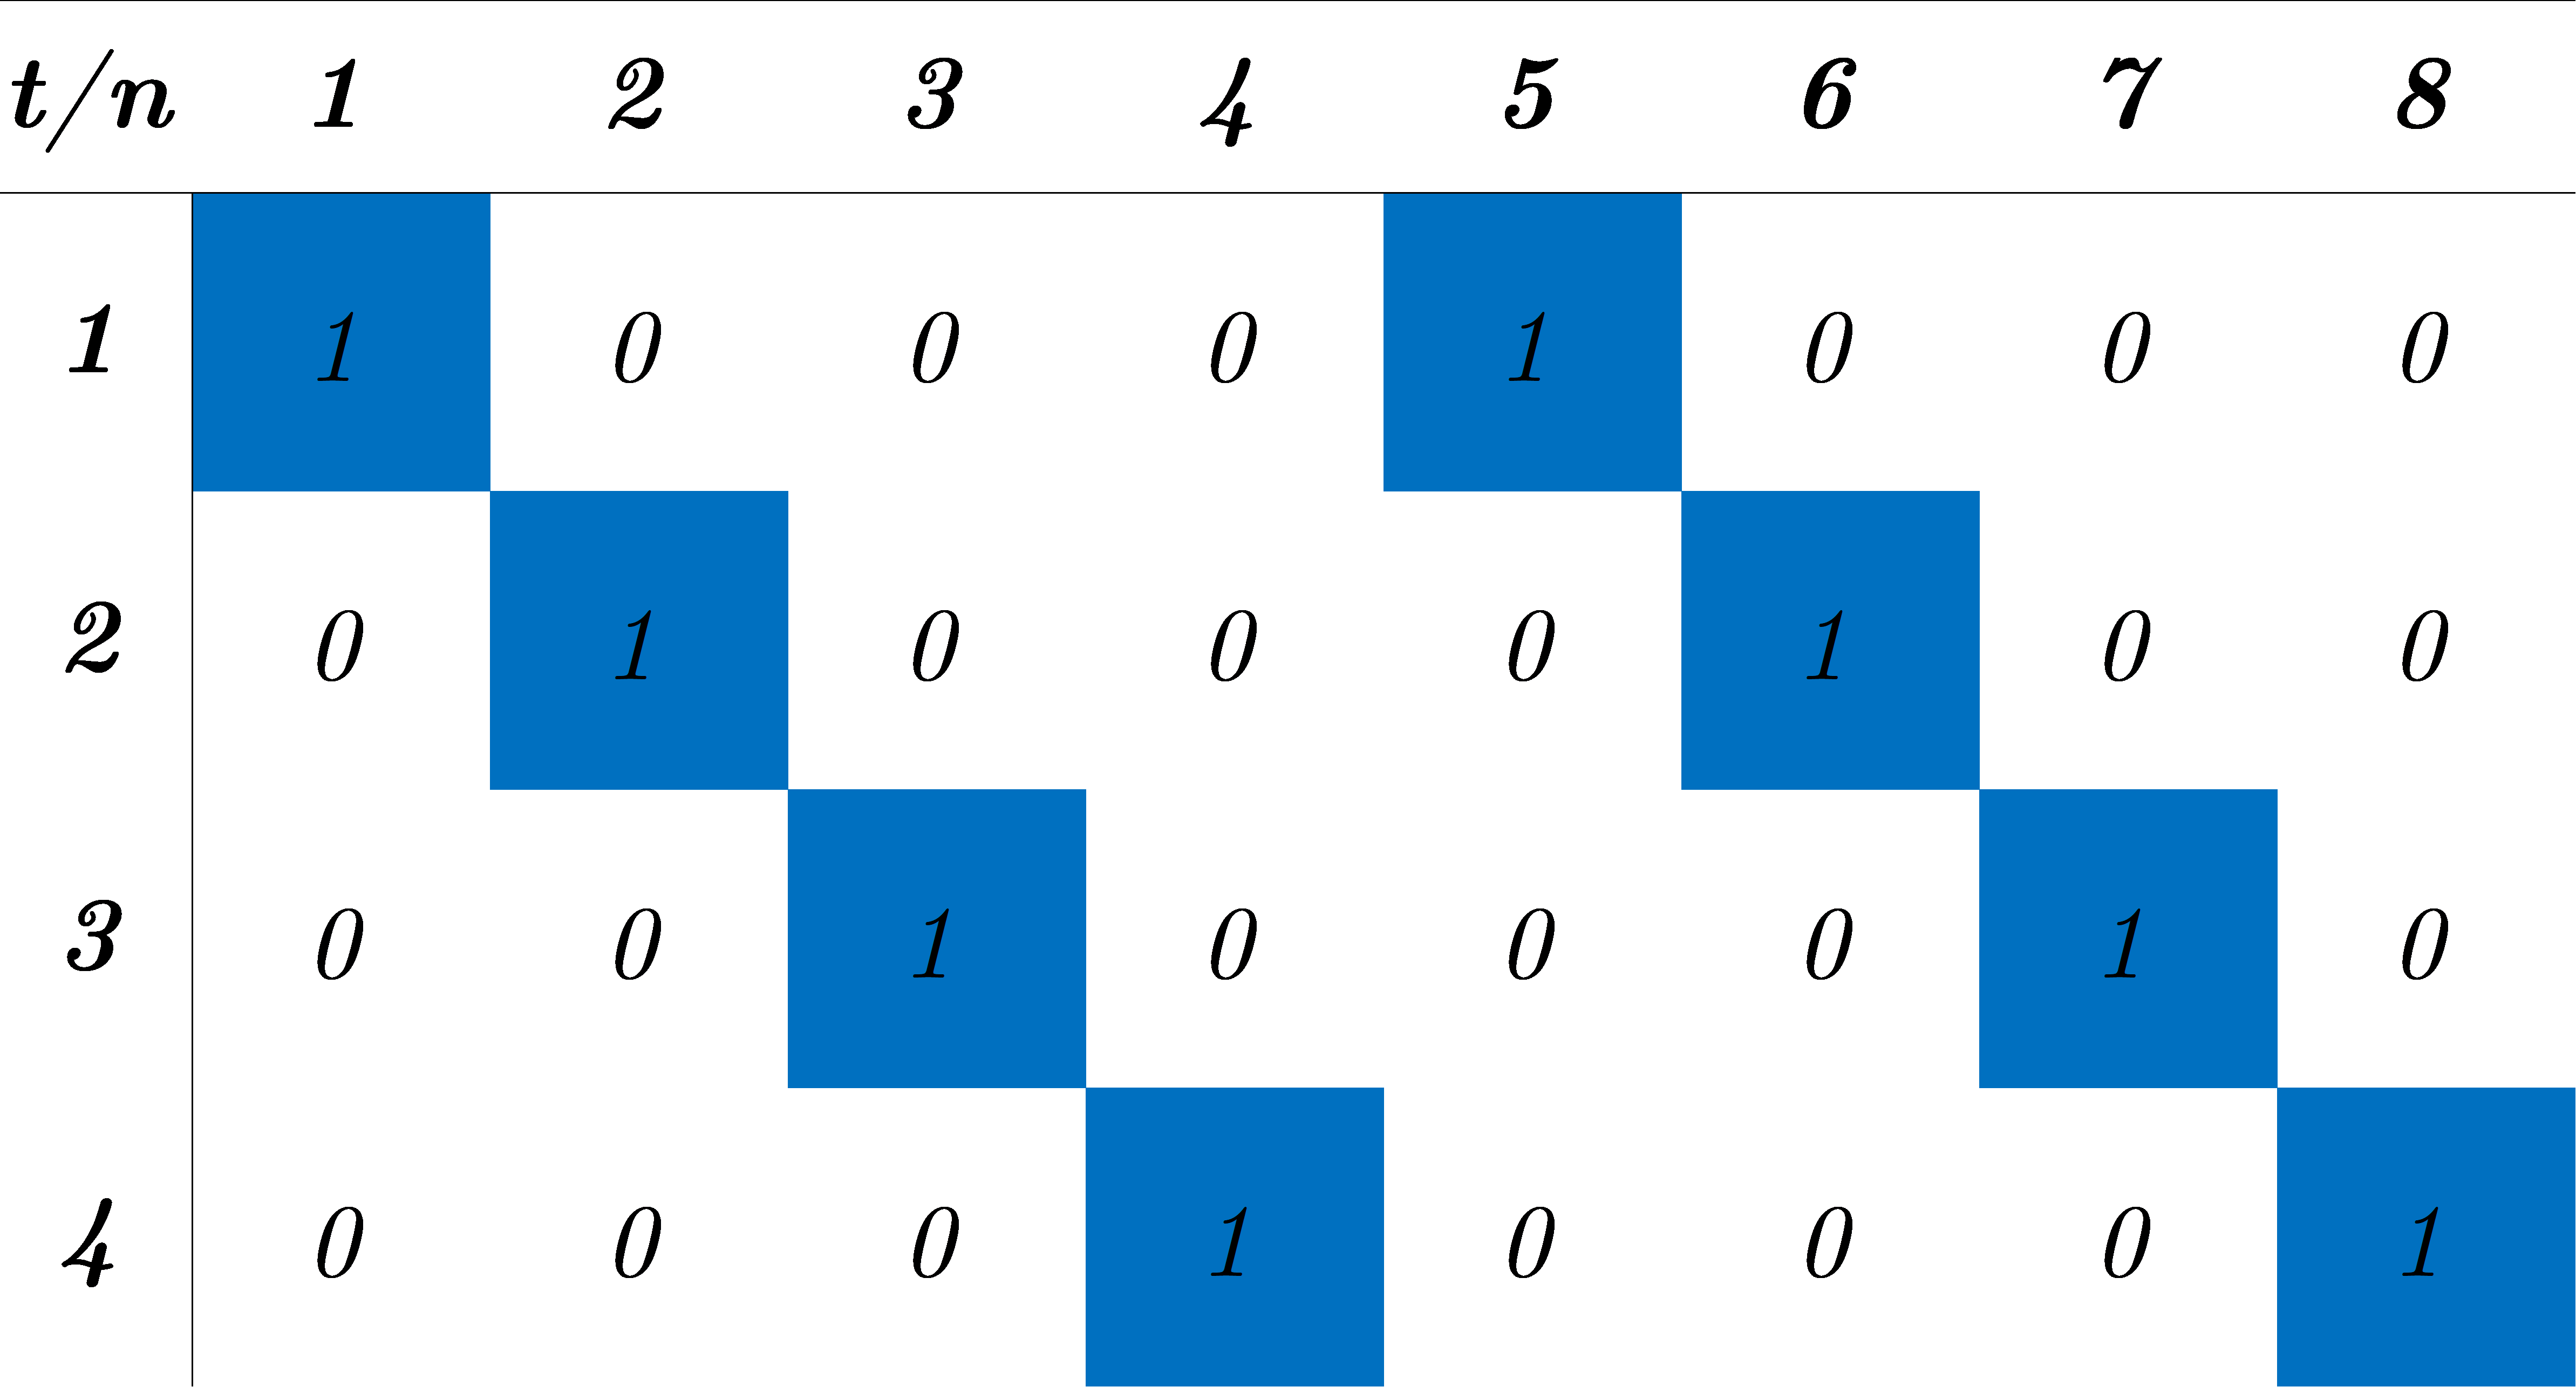
\includegraphics[width=10cm]{Figures/testsxexaminees.png}
	\caption{An example of \emph{tests $\times$ examinees} design, for $T=4$ tests, and $N=8$ test takers. }
	\label{fig:testsxexaminees}
\end{figure}
\pagebreak

\begin{figure}[H] 
	\centering
	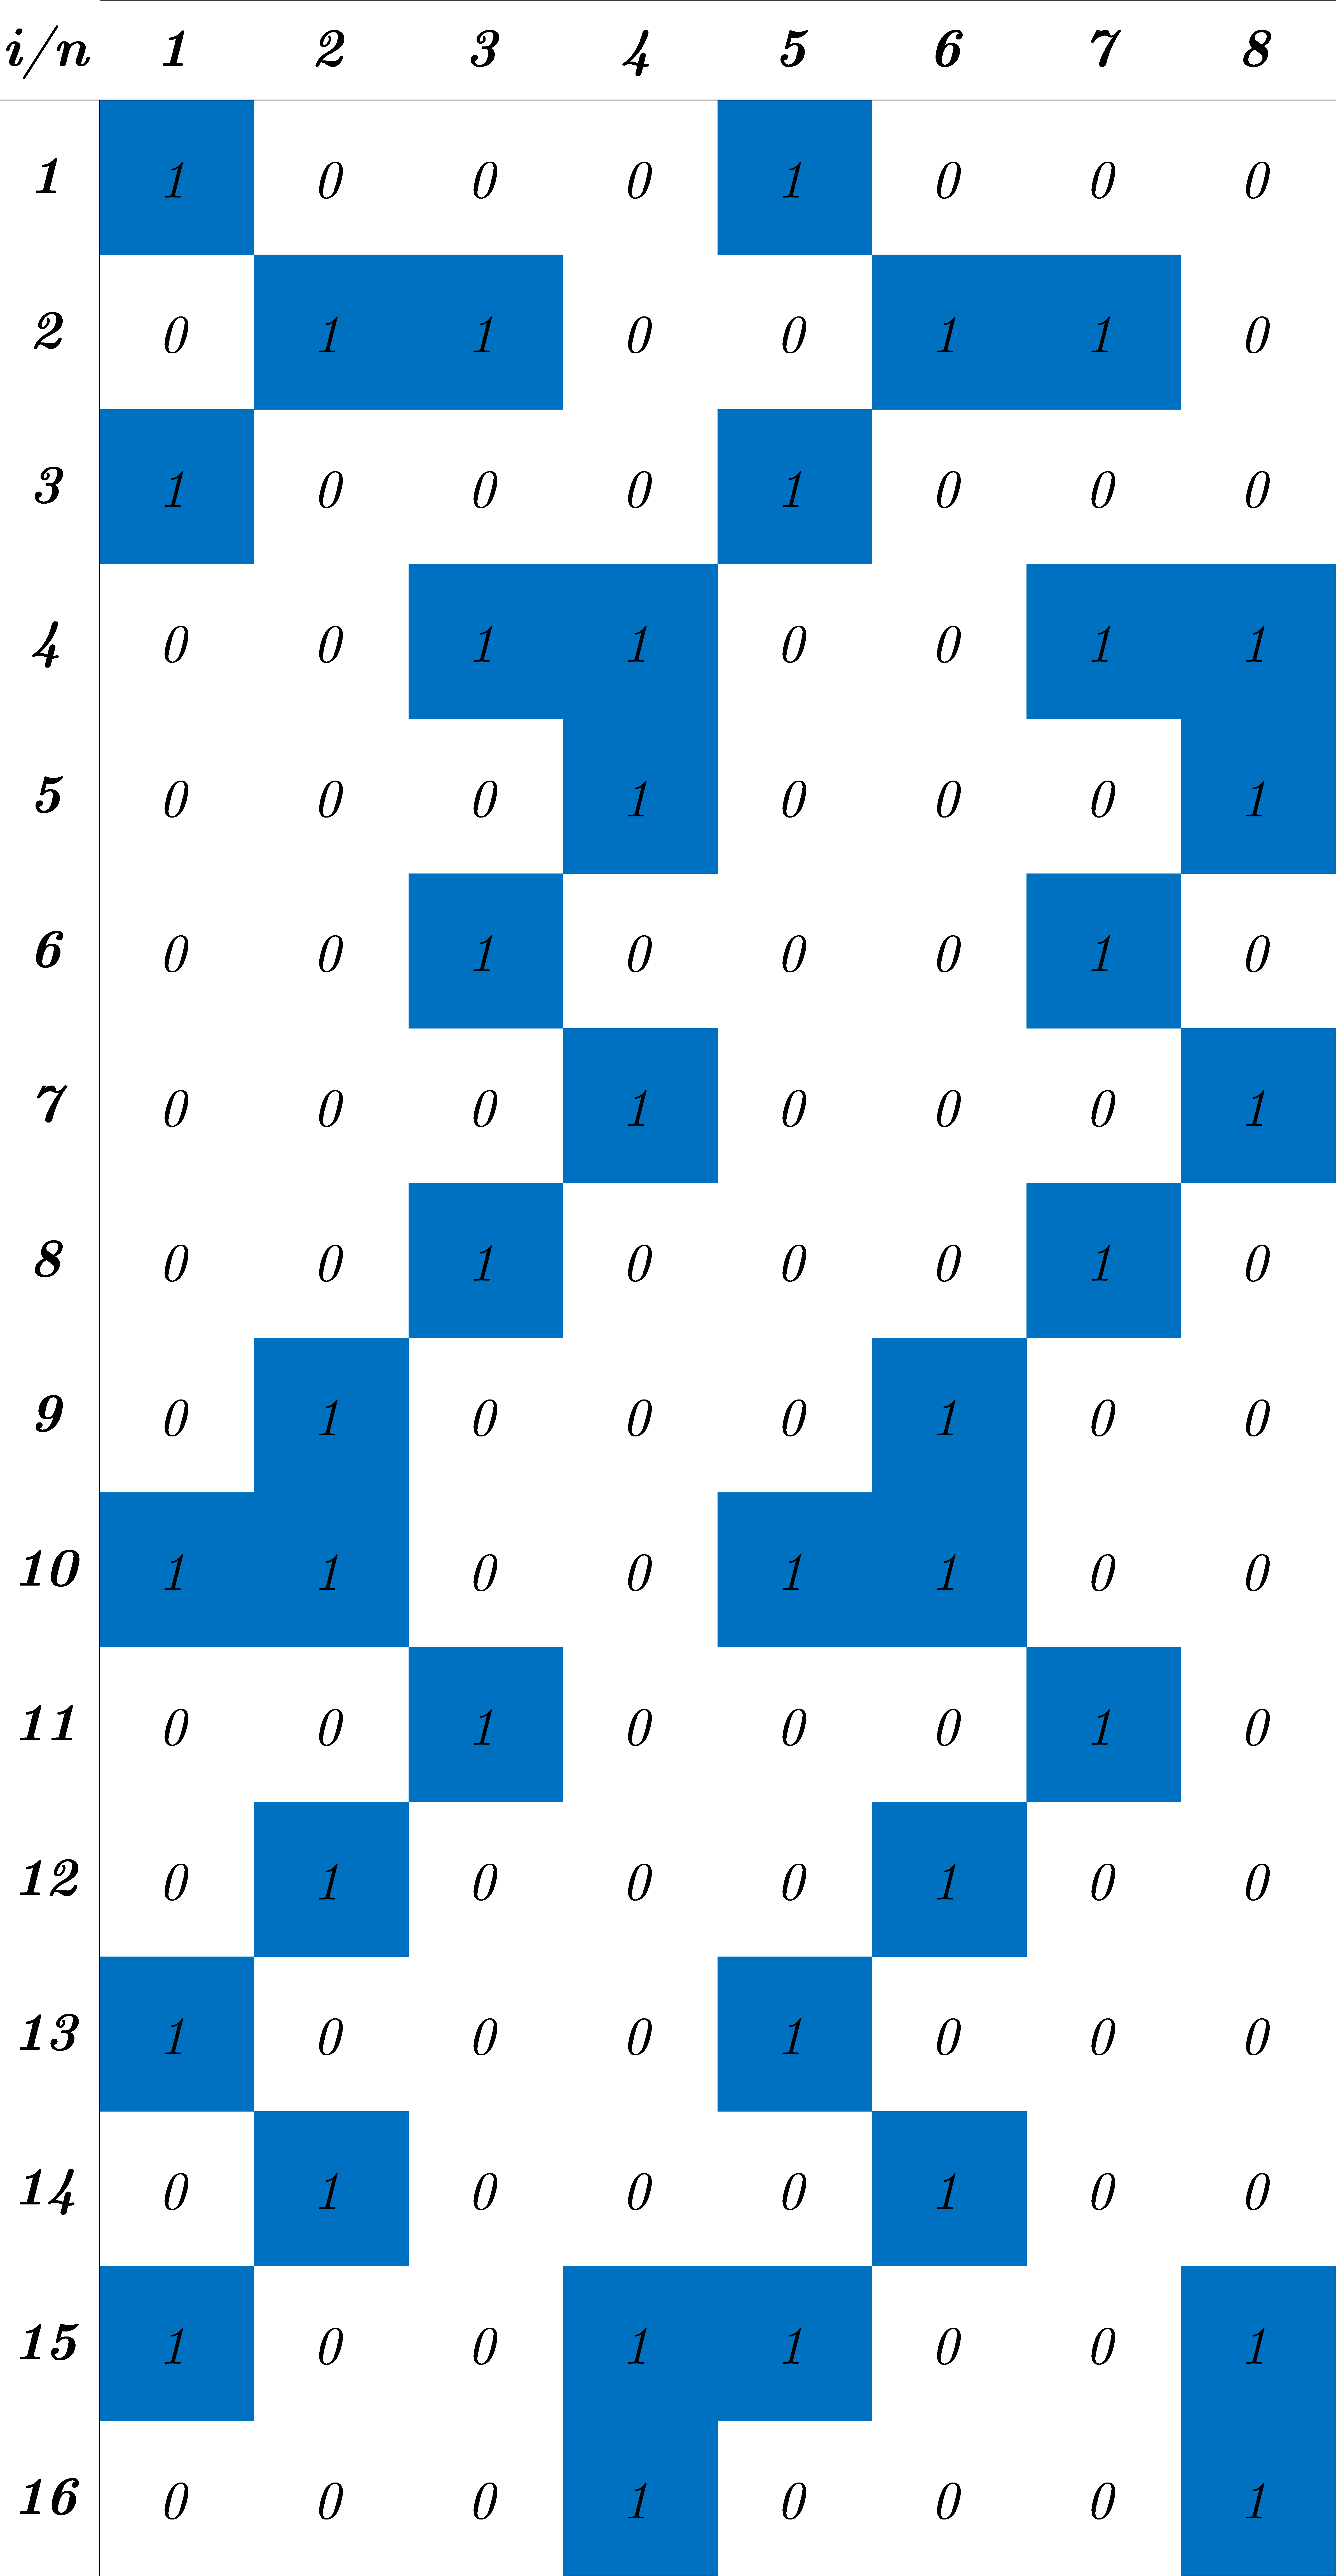
\includegraphics[width=10cm]{Figures/itemsxexaminees.png}
	\caption{An example of \emph{items $\times$ examinees} design, for $I=16$ items, and $N=8$ test takers.}
	\label{fig:itemsxexaminees}
\end{figure}
\pagebreak

\section{Items calibration in Julia}
\subsection{Case 1a (Standard setup)}

\begin{table}[H]
	\caption{Case 1a - RMSE and BIAS of item parameters averaged across the simulations, part 1/5}
	\def\arraystretch{0.9}
	\centering 	
	\resizebox{\textwidth}{!}{
		\begin{tabular}{l|c|ccc|ccc|c|ccc|ccc}
			\toprule
			& &\multicolumn{3}{c|}{b RMSE} & \multicolumn{3}{c|}{b BIAS} &  &\multicolumn{3}{c|}{a RMSE} & \multicolumn{3}{c}{a BIAS}\\
			i & $b^\dagger$ & jl & mirt & mirt\tiny{EHW} & jl & mirt & mirt\tiny{EHW} & $a^\dagger$ & jl & mirt & mirt\tiny{EHW} & jl & mirt & mirt\tiny{EHW} \\
			\midrule
			
			1 & -1.942 & 0.09 & 0.089 & 0.09 & -0.018 & -0.014 & -0.018 & 0.893 & 0.111 & 0.112 & 0.111 & -0.015 & -0.015 & -0.014 \\
			2 & -0.704 & 0.095 & 0.094 & 0.095 & -0.022 & -0.019 & -0.022 & 0.805 & 0.117 & 0.117 & 0.117 & -0.017 & -0.014 & -0.017 \\
			3 & -0.842 & 0.084 & 0.084 & 0.084 & -0.02 & -0.017 & -0.02 & 0.963 & 0.098 & 0.099 & 0.098 & -0.023 & -0.02 & -0.023 \\
			4 & -0.502 & 0.09 & 0.09 & 0.09 & 0.044 & 0.045 & 0.045 & 0.838 & 0.071 & 0.072 & 0.071 & 0.003 & 0.003 & 0.004 \\
			5 & 1.104 & 0.1 & 0.098 & 0.1 & -0.039 & -0.036 & -0.039 & 1.12 & 0.104 & 0.104 & 0.104 & 0.006 & 0.008 & 0.007 \\
			6 & -0.625 & 0.077 & 0.075 & 0.077 & -0.027 & -0.023 & -0.026 & 1.297 & 0.106 & 0.105 & 0.106 & -0.043 & -0.037 & -0.042 \\
			7 & -0.39 & 0.073 & 0.072 & 0.073 & -0.015 & -0.011 & -0.015 & 1.035 & 0.09 & 0.09 & 0.09 & -0.032 & -0.028 & -0.031 \\
			8 & 0.077 & 0.087 & 0.086 & 0.087 & -0.03 & -0.026 & -0.03 & 1.457 & 0.116 & 0.115 & 0.116 & -0.038 & -0.03 & -0.037 \\
			9 & -1.368 & 0.093 & 0.092 & 0.093 & -0.019 & -0.015 & -0.019 & 1.059 & 0.105 & 0.106 & 0.104 & -0.015 & -0.012 & -0.014 \\
			10 & -0.437 & 0.086 & 0.084 & 0.086 & -0.041 & -0.037 & -0.041 & 1.031 & 0.101 & 0.102 & 0.102 & 0.006 & 0.01 & 0.007 \\
			11 & -1.4 & 0.1 & 0.099 & 0.1 & -0.03 & -0.026 & -0.03 & 1.094 & 0.101 & 0.101 & 0.101 & -0.018 & -0.014 & -0.016 \\
			12 & -0.617 & 0.087 & 0.086 & 0.087 & -0.033 & -0.03 & -0.033 & 0.903 & 0.085 & 0.085 & 0.085 & -0.022 & -0.019 & -0.022 \\
			13 & -0.068 & 0.078 & 0.077 & 0.078 & -0.016 & -0.014 & -0.016 & 0.55 & 0.084 & 0.084 & 0.084 & 0.012 & 0.013 & 0.012 \\
			14 & 1.432 & 0.101 & 0.1 & 0.101 & -0.039 & -0.036 & -0.039 & 1.033 & 0.106 & 0.105 & 0.106 & -0.024 & -0.022 & -0.022 \\
			15 & -0.379 & 0.08 & 0.079 & 0.08 & -0.02 & -0.017 & -0.02 & 0.893 & 0.096 & 0.097 & 0.097 & -0.009 & -0.005 & -0.008 \\
			16 & -1.547 & 0.104 & 0.103 & 0.103 & -0.026 & -0.021 & -0.026 & 1.402 & 0.136 & 0.134 & 0.134 & -0.062 & -0.055 & -0.059 \\
			17 & -0.628 & 0.09 & 0.088 & 0.091 & -0.037 & -0.034 & -0.037 & 1.086 & 0.099 & 0.101 & 0.099 & 0.024 & 0.029 & 0.026 \\
			18 & -0.023 & 0.085 & 0.084 & 0.085 & -0.025 & -0.022 & -0.026 & 1.162 & 0.099 & 0.101 & 0.1 & 0.002 & 0.007 & 0.003 \\
			19 & 0.051 & 0.073 & 0.072 & 0.073 & -0.029 & -0.027 & -0.029 & 0.811 & 0.088 & 0.088 & 0.088 & -0.03 & -0.027 & -0.029 \\
			20 & 0.906 & 0.07 & 0.069 & 0.07 & -0.019 & -0.017 & -0.019 & 0.701 & 0.086 & 0.086 & 0.087 & 0.002 & 0.003 & 0.003 \\
			21 & -2.054 & 0.13 & 0.13 & 0.13 & 0.015 & 0.019 & 0.015 & 1.057 & 0.114 & 0.114 & 0.114 & 0.009 & 0.007 & 0.011 \\
			22 & 1.0 & 0.092 & 0.092 & 0.092 & 0.014 & 0.016 & 0.015 & 1.225 & 0.109 & 0.11 & 0.11 & 0.004 & 0.005 & 0.006 \\
			23 & 0.963 & 0.113 & 0.112 & 0.113 & -0.028 & -0.025 & -0.028 & 0.978 & 0.119 & 0.119 & 0.119 & 0.019 & 0.021 & 0.02 \\
			24 & 0.013 & 0.07 & 0.07 & 0.07 & 0.017 & 0.019 & 0.018 & 1.323 & 0.107 & 0.109 & 0.108 & 0.023 & 0.028 & 0.025 \\
			25 & 1.543 & 0.12 & 0.119 & 0.12 & -0.038 & -0.035 & -0.037 & 1.514 & 0.137 & 0.136 & 0.136 & -0.027 & -0.025 & -0.026 \\
			26 & 0.697 & 0.081 & 0.081 & 0.081 & 0.046 & 0.047 & 0.047 & 1.177 & 0.101 & 0.101 & 0.103 & 0.012 & 0.012 & 0.014 \\
			27 & -0.456 & 0.131 & 0.13 & 0.131 & -0.033 & -0.029 & -0.033 & 1.24 & 0.147 & 0.149 & 0.148 & 0.027 & 0.034 & 0.029 \\
			28 & -1.062 & 0.121 & 0.121 & 0.121 & -0.006 & -0.002 & -0.005 & 1.152 & 0.133 & 0.134 & 0.134 & -0.016 & -0.013 & -0.015 \\
			29 & 2.575 & 0.155 & 0.155 & 0.155 & -0.017 & -0.015 & -0.017 & 1.079 & 0.147 & 0.146 & 0.148 & 0.023 & 0.023 & 0.025 \\
			30 & -0.251 & 0.081 & 0.081 & 0.081 & 0.011 & 0.013 & 0.012 & 1.222 & 0.098 & 0.099 & 0.099 & 0.007 & 0.011 & 0.008 \\
			31 & 1.672 & 0.091 & 0.092 & 0.091 & 0.042 & 0.042 & 0.042 & 0.938 & 0.089 & 0.089 & 0.09 & 0.03 & 0.029 & 0.032 \\
			32 & -1.746 & 0.124 & 0.123 & 0.124 & -0.03 & -0.025 & -0.03 & 1.244 & 0.117 & 0.117 & 0.117 & -0.028 & -0.025 & -0.027 \\
			33 & -0.363 & 0.076 & 0.077 & 0.077 & 0.03 & 0.03 & 0.03 & 0.934 & 0.093 & 0.093 & 0.093 & 0.006 & 0.007 & 0.008 \\
			34 & 0.509 & 0.067 & 0.067 & 0.067 & -0.005 & -0.003 & -0.005 & 0.826 & 0.089 & 0.089 & 0.088 & -0.014 & -0.011 & -0.013 \\
			35 & -0.691 & 0.11 & 0.109 & 0.11 & -0.022 & -0.019 & -0.022 & 1.104 & 0.146 & 0.148 & 0.146 & -0.003 & 0.002 & -0.001 \\
			36 & -0.517 & 0.088 & 0.086 & 0.088 & -0.042 & -0.038 & -0.042 & 1.169 & 0.1 & 0.103 & 0.1 & 0.028 & 0.034 & 0.03 \\
			37 & 1.565 & 0.111 & 0.112 & 0.111 & 0.024 & 0.025 & 0.025 & 1.176 & 0.112 & 0.111 & 0.113 & 0.027 & 0.027 & 0.029 \\
			38 & -0.464 & 0.109 & 0.109 & 0.109 & 0.016 & 0.018 & 0.017 & 1.203 & 0.143 & 0.145 & 0.144 & 0.036 & 0.039 & 0.038 \\
			39 & 0.396 & 0.117 & 0.115 & 0.117 & -0.041 & -0.037 & -0.04 & 1.155 & 0.139 & 0.139 & 0.14 & -0.024 & -0.018 & -0.022 \\
			40 & -0.291 & 0.138 & 0.138 & 0.138 & 0.09 & 0.09 & 0.091 & 1.453 & 0.177 & 0.178 & 0.178 & 0.041 & 0.046 & 0.043 \\
			41 & -0.24 & 0.115 & 0.114 & 0.115 & -0.034 & -0.03 & -0.034 & 1.413 & 0.149 & 0.148 & 0.149 & -0.038 & -0.029 & -0.037 \\
			42 & 0.749 & 0.092 & 0.091 & 0.092 & -0.017 & -0.014 & -0.017 & 1.306 & 0.115 & 0.115 & 0.114 & -0.022 & -0.018 & -0.021 \\
			43 & -1.447 & 0.131 & 0.129 & 0.131 & -0.042 & -0.039 & -0.042 & 0.941 & 0.171 & 0.171 & 0.171 & -0.044 & -0.04 & -0.043 \\
			44 & -0.835 & 0.103 & 0.103 & 0.103 & -0.025 & -0.023 & -0.025 & 0.654 & 0.115 & 0.115 & 0.115 & -0.009 & -0.008 & -0.008 \\
			45 & 1.481 & 0.121 & 0.121 & 0.121 & 0.021 & 0.023 & 0.021 & 0.817 & 0.141 & 0.141 & 0.141 & 0.004 & 0.005 & 0.004 \\
			46 & 2.0 & 0.123 & 0.122 & 0.123 & -0.017 & -0.015 & -0.017 & 1.026 & 0.122 & 0.122 & 0.123 & 0.006 & 0.006 & 0.008 \\
			47 & -0.488 & 0.082 & 0.081 & 0.082 & 0.004 & 0.006 & 0.004 & 0.865 & 0.101 & 0.102 & 0.102 & 0.014 & 0.016 & 0.015 \\
			48 & 1.146 & 0.086 & 0.086 & 0.086 & 0.018 & 0.02 & 0.019 & 0.937 & 0.093 & 0.093 & 0.092 & -0.011 & -0.01 & -0.009 \\
			49 & -0.26 & 0.111 & 0.11 & 0.111 & -0.026 & -0.023 & -0.026 & 1.044 & 0.113 & 0.115 & 0.113 & 0.003 & 0.007 & 0.005 \\
			50 & -0.016 & 0.09 & 0.091 & 0.09 & 0.002 & 0.004 & 0.002 & 0.737 & 0.109 & 0.11 & 0.11 & 0.01 & 0.012 & 0.011 \\
	\end{tabular}}
	
\end{table}
\pagebreak
\begin{table}[H]
	\caption{Case 1a - RMSE and BIAS of item parameters averaged across the simulations, part 2/5}
	\def\arraystretch{0.9}
	\centering 	\resizebox{\textwidth}{!}{
		\begin{tabular}{l|c|ccc|ccc|c|ccc|ccc}
			\toprule
			& &\multicolumn{3}{c|}{b RMSE} & \multicolumn{3}{c|}{b BIAS} &  &\multicolumn{3}{c|}{a RMSE} & \multicolumn{3}{c}{a BIAS}\\
			i & $b^\dagger$ & jl & mirt & mirt\tiny{EHW} & jl & mirt & mirt\tiny{EHW} & $a^\dagger$ & jl & mirt & mirt\tiny{EHW} & jl & mirt & mirt\tiny{EHW} \\
			\midrule
			
			51 & -2.564 & 0.19 & 0.189 & 0.19 & 0.025 & 0.028 & 0.026 & 0.794 & 0.163 & 0.159 & 0.164 & 0.029 & 0.023 & 0.029 \\
			52 & -1.078 & 0.122 & 0.122 & 0.122 & 0.039 & 0.04 & 0.04 & 0.863 & 0.122 & 0.122 & 0.123 & 0.035 & 0.034 & 0.036 \\
			53 & -1.115 & 0.124 & 0.125 & 0.125 & 0.062 & 0.063 & 0.063 & 1.067 & 0.14 & 0.14 & 0.141 & 0.01 & 0.011 & 0.012 \\
			54 & -0.156 & 0.131 & 0.131 & 0.132 & 0.075 & 0.075 & 0.076 & 1.078 & 0.138 & 0.139 & 0.138 & 0.048 & 0.049 & 0.049 \\
			55 & 1.776 & 0.165 & 0.164 & 0.165 & 0.081 & 0.081 & 0.082 & 0.945 & 0.162 & 0.162 & 0.163 & 0.031 & 0.029 & 0.032 \\
			56 & 0.452 & 0.089 & 0.09 & 0.089 & 0.053 & 0.053 & 0.053 & 1.22 & 0.084 & 0.086 & 0.085 & 0.037 & 0.039 & 0.039 \\
			57 & -0.757 & 0.146 & 0.146 & 0.147 & 0.086 & 0.087 & 0.087 & 1.154 & 0.148 & 0.15 & 0.148 & 0.03 & 0.032 & 0.032 \\
			58 & -0.763 & 0.128 & 0.127 & 0.128 & -0.015 & -0.011 & -0.015 & 1.042 & 0.137 & 0.138 & 0.138 & 0.027 & 0.031 & 0.028 \\
			59 & 1.02 & 0.104 & 0.103 & 0.104 & -0.018 & -0.015 & -0.018 & 0.853 & 0.127 & 0.128 & 0.127 & 0.034 & 0.036 & 0.035 \\
			60 & -0.4 & 0.101 & 0.1 & 0.101 & -0.024 & -0.022 & -0.025 & 0.711 & 0.104 & 0.105 & 0.104 & 0.022 & 0.024 & 0.022 \\
			61 & 0.625 & 0.107 & 0.107 & 0.107 & -0.008 & -0.005 & -0.009 & 1.185 & 0.145 & 0.147 & 0.145 & 0.029 & 0.033 & 0.031 \\
			62 & -0.325 & 0.098 & 0.097 & 0.098 & -0.021 & -0.019 & -0.021 & 0.649 & 0.109 & 0.11 & 0.11 & 0.035 & 0.037 & 0.036 \\
			63 & -1.807 & 0.157 & 0.156 & 0.157 & -0.048 & -0.044 & -0.048 & 0.796 & 0.164 & 0.164 & 0.166 & 0.037 & 0.036 & 0.037 \\
			64 & -0.4 & 0.106 & 0.106 & 0.106 & -0.013 & -0.009 & -0.013 & 1.081 & 0.134 & 0.136 & 0.133 & 0.027 & 0.031 & 0.028 \\
			65 & 0.824 & 0.111 & 0.11 & 0.11 & -0.02 & -0.017 & -0.021 & 1.228 & 0.157 & 0.158 & 0.158 & 0.04 & 0.044 & 0.041 \\
			66 & 0.577 & 0.112 & 0.111 & 0.112 & -0.027 & -0.024 & -0.028 & 1.157 & 0.17 & 0.172 & 0.172 & 0.05 & 0.053 & 0.051 \\
			67 & -0.896 & 0.117 & 0.117 & 0.117 & 0.057 & 0.058 & 0.057 & 0.942 & 0.134 & 0.134 & 0.135 & 0.027 & 0.027 & 0.029 \\
			68 & -0.425 & 0.144 & 0.144 & 0.144 & 0.083 & 0.084 & 0.084 & 1.172 & 0.161 & 0.163 & 0.16 & 0.03 & 0.033 & 0.032 \\
			69 & -1.95 & 0.171 & 0.17 & 0.171 & 0.041 & 0.043 & 0.042 & 0.882 & 0.16 & 0.159 & 0.161 & 0.04 & 0.036 & 0.042 \\
			70 & 0.815 & 0.151 & 0.152 & 0.152 & 0.075 & 0.075 & 0.076 & 1.023 & 0.136 & 0.136 & 0.136 & 0.024 & 0.024 & 0.025 \\
			71 & 0.16 & 0.108 & 0.108 & 0.109 & -0.034 & -0.031 & -0.034 & 1.047 & 0.135 & 0.136 & 0.135 & 0.013 & 0.017 & 0.015 \\
			72 & 0.164 & 0.092 & 0.092 & 0.092 & -0.012 & -0.009 & -0.011 & 0.759 & 0.104 & 0.105 & 0.105 & -0.008 & -0.006 & -0.007 \\
			73 & -0.651 & 0.101 & 0.101 & 0.101 & -0.019 & -0.017 & -0.019 & 0.736 & 0.105 & 0.106 & 0.105 & 0.011 & 0.013 & 0.011 \\
			74 & 0.042 & 0.1 & 0.1 & 0.101 & -0.009 & -0.006 & -0.009 & 0.851 & 0.133 & 0.133 & 0.133 & -0.029 & -0.025 & -0.028 \\
			75 & 0.653 & 0.108 & 0.108 & 0.108 & -0.026 & -0.023 & -0.025 & 0.879 & 0.122 & 0.121 & 0.122 & -0.028 & -0.025 & -0.027 \\
			76 & -0.765 & 0.087 & 0.086 & 0.087 & -0.028 & -0.027 & -0.028 & 0.408 & 0.122 & 0.122 & 0.122 & -0.002 & -0.001 & -0.002 \\
			77 & 0.729 & 0.106 & 0.106 & 0.106 & 0.005 & 0.007 & 0.004 & 0.787 & 0.126 & 0.127 & 0.126 & 0.029 & 0.031 & 0.03 \\
			78 & -2.147 & 0.146 & 0.144 & 0.145 & -0.033 & -0.028 & -0.032 & 1.208 & 0.173 & 0.172 & 0.174 & 0.048 & 0.044 & 0.051 \\
			79 & -0.702 & 0.109 & 0.108 & 0.109 & -0.036 & -0.033 & -0.037 & 0.979 & 0.12 & 0.122 & 0.12 & 0.029 & 0.033 & 0.03 \\
			80 & -1.629 & 0.139 & 0.138 & 0.139 & -0.042 & -0.039 & -0.042 & 0.65 & 0.138 & 0.139 & 0.138 & -0.01 & -0.009 & -0.01 \\
			81 & -0.408 & 0.118 & 0.116 & 0.118 & -0.037 & -0.034 & -0.038 & 1.251 & 0.155 & 0.158 & 0.154 & 0.022 & 0.029 & 0.023 \\
			82 & -0.948 & 0.114 & 0.113 & 0.115 & -0.017 & -0.013 & -0.017 & 0.971 & 0.144 & 0.146 & 0.144 & 0.01 & 0.014 & 0.011 \\
			83 & 0.62 & 0.106 & 0.106 & 0.106 & 0.032 & 0.033 & 0.033 & 0.741 & 0.123 & 0.124 & 0.125 & 0.027 & 0.028 & 0.029 \\
			84 & 1.187 & 0.116 & 0.115 & 0.116 & -0.008 & -0.005 & -0.007 & 0.92 & 0.154 & 0.155 & 0.154 & -0.004 & -0.002 & -0.002 \\
			85 & -2.191 & 0.21 & 0.204 & 0.211 & -0.041 & -0.033 & -0.042 & 1.416 & 0.2 & 0.2 & 0.2 & 0.013 & 0.013 & 0.014 \\
			86 & 0.467 & 0.11 & 0.11 & 0.111 & -0.018 & -0.015 & -0.018 & 0.997 & 0.119 & 0.12 & 0.12 & 0.015 & 0.018 & 0.016 \\
			87 & 0.865 & 0.117 & 0.117 & 0.117 & -0.005 & -0.002 & -0.005 & 1.022 & 0.151 & 0.153 & 0.152 & 0.053 & 0.056 & 0.054 \\
			88 & -0.745 & 0.108 & 0.108 & 0.108 & -0.003 & 0.0 & -0.003 & 1.308 & 0.148 & 0.15 & 0.147 & -0.001 & 0.005 & 0.0 \\
			89 & 1.071 & 0.125 & 0.125 & 0.125 & 0.028 & 0.028 & 0.028 & 1.029 & 0.144 & 0.144 & 0.145 & 0.007 & 0.007 & 0.01 \\
			90 & 0.124 & 0.113 & 0.113 & 0.113 & -0.035 & -0.032 & -0.035 & 0.985 & 0.123 & 0.124 & 0.123 & -0.0 & 0.003 & 0.001 \\
			91 & 0.695 & 0.115 & 0.115 & 0.115 & 0.021 & 0.022 & 0.021 & 0.971 & 0.125 & 0.125 & 0.125 & 0.006 & 0.007 & 0.008 \\
			92 & 0.516 & 0.108 & 0.108 & 0.108 & 0.023 & 0.026 & 0.023 & 1.152 & 0.152 & 0.153 & 0.152 & -0.022 & -0.018 & -0.021 \\
			93 & -0.088 & 0.087 & 0.088 & 0.087 & 0.01 & 0.012 & 0.01 & 0.955 & 0.121 & 0.121 & 0.12 & -0.029 & -0.027 & -0.028 \\
			94 & 0.544 & 0.114 & 0.115 & 0.115 & 0.047 & 0.047 & 0.047 & 0.665 & 0.115 & 0.115 & 0.115 & 0.024 & 0.024 & 0.025 \\
			95 & -1.625 & 0.146 & 0.144 & 0.146 & -0.039 & -0.035 & -0.039 & 0.913 & 0.159 & 0.159 & 0.16 & -0.003 & -0.003 & -0.001 \\
			96 & 0.505 & 0.106 & 0.106 & 0.107 & -0.017 & -0.013 & -0.018 & 1.348 & 0.163 & 0.164 & 0.164 & 0.04 & 0.046 & 0.041 \\
			97 & 0.844 & 0.122 & 0.121 & 0.122 & -0.023 & -0.02 & -0.023 & 0.821 & 0.129 & 0.13 & 0.13 & 0.034 & 0.036 & 0.035 \\
			98 & 1.42 & 0.153 & 0.153 & 0.153 & 0.064 & 0.064 & 0.065 & 0.977 & 0.131 & 0.13 & 0.131 & -0.006 & -0.007 & -0.005 \\
			99 & -0.409 & 0.121 & 0.12 & 0.122 & -0.026 & -0.022 & -0.026 & 1.187 & 0.158 & 0.161 & 0.159 & 0.052 & 0.058 & 0.053 \\
			100 & -0.525 & 0.117 & 0.116 & 0.117 & -0.035 & -0.032 & -0.036 & 1.054 & 0.141 & 0.144 & 0.142 & 0.034 & 0.039 & 0.036 \\
	\end{tabular}}
	
\end{table}
\pagebreak
\begin{table}[H]
	\caption{Case 1a - RMSE and BIAS of item parameters averaged across the simulations, part 3/5}
	\def\arraystretch{0.9}
	\centering 	\resizebox{\textwidth}{!}{
		\begin{tabular}{l|c|ccc|ccc|c|ccc|ccc}
			\toprule
			& &\multicolumn{3}{c|}{b RMSE} & \multicolumn{3}{c|}{b BIAS} &  &\multicolumn{3}{c|}{a RMSE} & \multicolumn{3}{c}{a BIAS}\\
			i & $b^\dagger$ & jl & mirt & mirt\tiny{EHW} & jl & mirt & mirt\tiny{EHW} & $a^\dagger$ & jl & mirt & mirt\tiny{EHW} & jl & mirt & mirt\tiny{EHW} \\
			\midrule
			
			101 & 0.648 & 0.108 & 0.108 & 0.108 & -0.025 & -0.021 & -0.025 & 1.574 & 0.192 & 0.193 & 0.192 & 0.015 & 0.022 & 0.017 \\
			102 & 0.342 & 0.111 & 0.11 & 0.111 & -0.029 & -0.026 & -0.029 & 1.019 & 0.138 & 0.138 & 0.138 & -0.032 & -0.028 & -0.032 \\
			103 & -1.121 & 0.163 & 0.163 & 0.163 & 0.087 & 0.088 & 0.087 & 1.363 & 0.174 & 0.178 & 0.175 & 0.06 & 0.064 & 0.062 \\
			104 & -0.354 & 0.11 & 0.109 & 0.11 & -0.018 & -0.014 & -0.018 & 1.083 & 0.148 & 0.151 & 0.149 & 0.008 & 0.012 & 0.009 \\
			105 & 0.302 & 0.075 & 0.075 & 0.075 & -0.007 & -0.004 & -0.006 & 0.851 & 0.086 & 0.086 & 0.086 & -0.017 & -0.014 & -0.016 \\
			106 & -0.535 & 0.119 & 0.117 & 0.12 & -0.027 & -0.023 & -0.028 & 1.236 & 0.161 & 0.165 & 0.161 & 0.036 & 0.042 & 0.037 \\
			107 & 0.156 & 0.09 & 0.089 & 0.09 & -0.033 & -0.031 & -0.033 & 0.646 & 0.108 & 0.108 & 0.108 & -0.021 & -0.019 & -0.021 \\
			108 & 1.033 & 0.111 & 0.111 & 0.111 & -0.008 & -0.006 & -0.008 & 0.753 & 0.144 & 0.145 & 0.145 & 0.037 & 0.039 & 0.038 \\
			109 & -1.446 & 0.122 & 0.121 & 0.122 & -0.016 & -0.015 & -0.016 & 0.746 & 0.137 & 0.136 & 0.138 & 0.039 & 0.038 & 0.041 \\
			110 & -2.571 & 0.223 & 0.22 & 0.224 & -0.024 & -0.017 & -0.024 & 1.02 & 0.225 & 0.224 & 0.225 & -0.024 & -0.028 & -0.024 \\
			111 & 0.627 & 0.095 & 0.094 & 0.095 & -0.014 & -0.013 & -0.014 & 0.624 & 0.106 & 0.107 & 0.107 & 0.005 & 0.006 & 0.006 \\
			112 & 0.855 & 0.183 & 0.182 & 0.184 & 0.116 & 0.116 & 0.118 & 1.758 & 0.204 & 0.204 & 0.204 & 0.014 & 0.016 & 0.016 \\
			113 & -1.154 & 0.168 & 0.166 & 0.169 & -0.066 & -0.061 & -0.067 & 1.482 & 0.212 & 0.219 & 0.213 & 0.083 & 0.093 & 0.084 \\
			114 & 1.02 & 0.104 & 0.104 & 0.104 & -0.001 & 0.001 & -0.001 & 0.593 & 0.125 & 0.124 & 0.125 & -0.013 & -0.012 & -0.013 \\
			115 & 0.851 & 0.106 & 0.106 & 0.106 & -0.012 & -0.01 & -0.012 & 0.933 & 0.146 & 0.147 & 0.147 & 0.023 & 0.026 & 0.025 \\
			116 & 0.88 & 0.127 & 0.127 & 0.127 & 0.008 & 0.01 & 0.008 & 0.839 & 0.146 & 0.146 & 0.146 & -0.015 & -0.014 & -0.014 \\
			117 & -0.924 & 0.136 & 0.134 & 0.135 & -0.048 & -0.044 & -0.048 & 1.098 & 0.164 & 0.166 & 0.164 & 0.049 & 0.053 & 0.05 \\
			118 & 1.09 & 0.126 & 0.125 & 0.126 & -0.032 & -0.029 & -0.032 & 1.213 & 0.135 & 0.135 & 0.135 & -0.018 & -0.015 & -0.017 \\
			119 & -0.833 & 0.102 & 0.101 & 0.102 & -0.014 & -0.011 & -0.014 & 1.02 & 0.145 & 0.145 & 0.145 & -0.047 & -0.042 & -0.046 \\
			120 & 0.48 & 0.091 & 0.091 & 0.091 & -0.021 & -0.018 & -0.021 & 0.707 & 0.108 & 0.108 & 0.108 & -0.028 & -0.026 & -0.027 \\
			121 & -0.074 & 0.096 & 0.096 & 0.096 & 0.013 & 0.014 & 0.014 & 0.795 & 0.103 & 0.103 & 0.104 & 0.017 & 0.017 & 0.019 \\
			122 & -0.808 & 0.124 & 0.124 & 0.124 & 0.029 & 0.031 & 0.03 & 0.994 & 0.146 & 0.147 & 0.147 & 0.013 & 0.015 & 0.015 \\
			123 & -1.243 & 0.136 & 0.136 & 0.136 & -0.025 & -0.021 & -0.026 & 1.103 & 0.142 & 0.144 & 0.142 & 0.031 & 0.034 & 0.031 \\
			124 & -0.524 & 0.116 & 0.116 & 0.116 & 0.003 & 0.005 & 0.004 & 1.309 & 0.156 & 0.159 & 0.157 & 0.047 & 0.051 & 0.049 \\
			125 & 0.002 & 0.092 & 0.092 & 0.092 & -0.013 & -0.01 & -0.013 & 0.893 & 0.125 & 0.126 & 0.125 & 0.013 & 0.015 & 0.014 \\
			126 & -0.355 & 0.097 & 0.097 & 0.097 & 0.013 & 0.014 & 0.014 & 0.705 & 0.114 & 0.114 & 0.114 & 0.005 & 0.005 & 0.007 \\
			127 & -0.575 & 0.1 & 0.1 & 0.1 & -0.001 & 0.001 & -0.001 & 0.672 & 0.106 & 0.107 & 0.106 & -0.007 & -0.006 & -0.006 \\
			128 & 1.402 & 0.144 & 0.145 & 0.145 & 0.02 & 0.022 & 0.02 & 1.021 & 0.154 & 0.154 & 0.154 & 0.017 & 0.018 & 0.019 \\
			129 & -0.337 & 0.109 & 0.108 & 0.109 & -0.04 & -0.036 & -0.04 & 0.976 & 0.152 & 0.155 & 0.153 & 0.049 & 0.053 & 0.05 \\
			130 & 0.495 & 0.121 & 0.121 & 0.121 & -0.028 & -0.024 & -0.027 & 1.384 & 0.149 & 0.151 & 0.149 & 0.017 & 0.023 & 0.019 \\
			131 & -0.293 & 0.094 & 0.093 & 0.094 & -0.014 & -0.012 & -0.014 & 0.689 & 0.115 & 0.115 & 0.115 & -0.037 & -0.035 & -0.036 \\
			132 & 0.841 & 0.105 & 0.105 & 0.105 & -0.017 & -0.014 & -0.016 & 0.886 & 0.148 & 0.149 & 0.148 & 0.018 & 0.02 & 0.02 \\
			133 & -1.18 & 0.113 & 0.112 & 0.113 & -0.032 & -0.03 & -0.032 & 0.676 & 0.119 & 0.119 & 0.12 & 0.005 & 0.007 & 0.007 \\
			134 & 1.117 & 0.11 & 0.11 & 0.11 & 0.026 & 0.026 & 0.026 & 1.027 & 0.157 & 0.157 & 0.158 & 0.047 & 0.047 & 0.049 \\
			135 & -0.275 & 0.102 & 0.101 & 0.102 & -0.023 & -0.02 & -0.023 & 0.922 & 0.133 & 0.133 & 0.133 & -0.037 & -0.033 & -0.036 \\
			136 & -0.629 & 0.104 & 0.104 & 0.105 & 0.001 & 0.002 & 0.001 & 0.699 & 0.122 & 0.122 & 0.122 & 0.016 & 0.016 & 0.018 \\
			137 & 1.167 & 0.128 & 0.126 & 0.128 & -0.053 & -0.049 & -0.053 & 1.403 & 0.169 & 0.169 & 0.169 & -0.048 & -0.044 & -0.047 \\
			138 & 0.589 & 0.107 & 0.107 & 0.107 & 0.024 & 0.025 & 0.024 & 0.868 & 0.144 & 0.144 & 0.145 & 0.02 & 0.021 & 0.022 \\
			139 & -0.431 & 0.095 & 0.096 & 0.095 & -0.002 & 0.001 & -0.002 & 0.869 & 0.131 & 0.131 & 0.131 & -0.006 & -0.003 & -0.005 \\
			140 & -0.481 & 0.102 & 0.103 & 0.103 & 0.026 & 0.027 & 0.026 & 1.007 & 0.122 & 0.123 & 0.122 & 0.031 & 0.032 & 0.033 \\
			141 & 0.407 & 0.114 & 0.114 & 0.115 & 0.063 & 0.064 & 0.064 & 0.908 & 0.124 & 0.124 & 0.124 & 0.022 & 0.022 & 0.023 \\
			142 & 1.198 & 0.091 & 0.091 & 0.091 & 0.028 & 0.029 & 0.028 & 0.902 & 0.105 & 0.105 & 0.106 & 0.031 & 0.031 & 0.032 \\
			143 & 1.97 & 0.19 & 0.19 & 0.191 & -0.021 & -0.018 & -0.021 & 1.256 & 0.175 & 0.175 & 0.176 & 0.036 & 0.037 & 0.037 \\
			144 & -1.514 & 0.136 & 0.134 & 0.136 & -0.034 & -0.029 & -0.034 & 1.354 & 0.189 & 0.188 & 0.188 & -0.076 & -0.069 & -0.074 \\
			145 & -0.594 & 0.103 & 0.103 & 0.103 & 0.012 & 0.013 & 0.012 & 1.069 & 0.131 & 0.132 & 0.132 & 0.014 & 0.015 & 0.016 \\
			146 & 0.685 & 0.119 & 0.119 & 0.119 & 0.037 & 0.038 & 0.037 & 1.06 & 0.14 & 0.141 & 0.141 & 0.046 & 0.047 & 0.048 \\
			147 & 1.502 & 0.14 & 0.14 & 0.14 & -0.001 & 0.002 & -0.001 & 1.253 & 0.183 & 0.183 & 0.184 & -0.021 & -0.019 & -0.02 \\
			148 & 0.268 & 0.089 & 0.088 & 0.089 & -0.029 & -0.027 & -0.029 & 0.825 & 0.116 & 0.116 & 0.117 & -0.009 & -0.007 & -0.008 \\
			149 & -0.742 & 0.107 & 0.107 & 0.107 & -0.002 & -0.0 & -0.001 & 1.367 & 0.157 & 0.16 & 0.157 & 0.03 & 0.034 & 0.032 \\
			150 & 0.955 & 0.117 & 0.115 & 0.117 & -0.018 & -0.015 & -0.018 & 1.047 & 0.136 & 0.137 & 0.136 & 0.036 & 0.039 & 0.038 \\
	\end{tabular}}
\end{table}
\pagebreak
\begin{table}[H]
	\caption{Case 1a - RMSE and BIAS of item parameters averaged across the simulations, part 4/5}
	\def\arraystretch{0.9}
	\centering 	\resizebox{\textwidth}{!}{
		\begin{tabular}{l|c|ccc|ccc|c|ccc|ccc}
			\toprule
			& &\multicolumn{3}{c|}{b RMSE} & \multicolumn{3}{c|}{b BIAS} &  &\multicolumn{3}{c|}{a RMSE} & \multicolumn{3}{c}{a BIAS}\\
			i & $b^\dagger$ & jl & mirt & mirt\tiny{EHW} & jl & mirt & mirt\tiny{EHW} & $a^\dagger$ & jl & mirt & mirt\tiny{EHW} & jl & mirt & mirt\tiny{EHW} \\
			\midrule
			
			151 & -0.769 & 0.116 & 0.115 & 0.116 & -0.024 & -0.022 & -0.025 & 0.648 & 0.128 & 0.128 & 0.128 & 0.017 & 0.017 & 0.017 \\
			152 & 0.702 & 0.106 & 0.105 & 0.107 & -0.031 & -0.027 & -0.031 & 1.295 & 0.15 & 0.15 & 0.15 & -0.036 & -0.03 & -0.035 \\
			153 & -0.216 & 0.1 & 0.099 & 0.1 & -0.021 & -0.019 & -0.022 & 0.655 & 0.121 & 0.121 & 0.12 & 0.016 & 0.017 & 0.017 \\
			154 & -0.975 & 0.114 & 0.112 & 0.114 & -0.026 & -0.023 & -0.027 & 0.988 & 0.153 & 0.155 & 0.154 & 0.047 & 0.05 & 0.048 \\
			155 & -1.306 & 0.123 & 0.123 & 0.123 & -0.003 & 0.0 & -0.003 & 1.019 & 0.146 & 0.148 & 0.147 & -0.019 & -0.017 & -0.018 \\
			156 & -1.22 & 0.131 & 0.131 & 0.131 & 0.023 & 0.025 & 0.023 & 1.135 & 0.167 & 0.168 & 0.168 & 0.024 & 0.024 & 0.026 \\
			157 & 0.777 & 0.14 & 0.141 & 0.141 & 0.084 & 0.084 & 0.085 & 1.316 & 0.159 & 0.159 & 0.16 & 0.002 & 0.003 & 0.003 \\
			158 & -0.375 & 0.111 & 0.111 & 0.111 & -0.02 & -0.017 & -0.02 & 1.72 & 0.185 & 0.188 & 0.186 & -0.012 & -0.0 & -0.012 \\
			159 & -0.077 & 0.124 & 0.122 & 0.124 & -0.034 & -0.03 & -0.034 & 1.645 & 0.165 & 0.163 & 0.166 & -0.046 & -0.035 & -0.045 \\
			160 & 0.581 & 0.097 & 0.097 & 0.097 & 0.01 & 0.01 & 0.01 & 0.612 & 0.112 & 0.112 & 0.112 & 0.018 & 0.018 & 0.02 \\
			161 & -1.697 & 0.149 & 0.148 & 0.148 & 0.014 & 0.018 & 0.014 & 0.934 & 0.159 & 0.158 & 0.16 & -0.035 & -0.035 & -0.034 \\
			162 & 0.255 & 0.119 & 0.12 & 0.12 & 0.041 & 0.042 & 0.042 & 1.354 & 0.165 & 0.166 & 0.166 & 0.047 & 0.049 & 0.049 \\
			163 & 2.141 & 0.198 & 0.198 & 0.198 & 0.04 & 0.042 & 0.041 & 1.444 & 0.203 & 0.202 & 0.203 & 0.003 & 0.002 & 0.005 \\
			164 & -0.082 & 0.105 & 0.105 & 0.105 & -0.012 & -0.009 & -0.012 & 1.015 & 0.118 & 0.12 & 0.119 & 0.004 & 0.008 & 0.006 \\
			165 & 0.53 & 0.087 & 0.087 & 0.087 & -0.02 & -0.017 & -0.019 & 0.743 & 0.122 & 0.122 & 0.121 & -0.027 & -0.025 & -0.026 \\
			166 & -0.082 & 0.109 & 0.109 & 0.109 & -0.003 & 0.001 & -0.003 & 1.109 & 0.155 & 0.155 & 0.154 & -0.04 & -0.034 & -0.039 \\
			167 & -0.053 & 0.106 & 0.105 & 0.106 & -0.015 & -0.012 & -0.015 & 1.145 & 0.136 & 0.137 & 0.136 & -0.002 & 0.002 & -0.001 \\
			168 & -0.401 & 0.104 & 0.104 & 0.103 & -0.013 & -0.011 & -0.013 & 0.717 & 0.118 & 0.119 & 0.118 & 0.006 & 0.008 & 0.007 \\
			169 & -0.994 & 0.12 & 0.119 & 0.12 & -0.039 & -0.036 & -0.039 & 1.088 & 0.142 & 0.144 & 0.142 & 0.004 & 0.008 & 0.005 \\
			170 & 0.656 & 0.117 & 0.117 & 0.118 & 0.069 & 0.069 & 0.07 & 1.05 & 0.133 & 0.133 & 0.133 & 0.039 & 0.04 & 0.04 \\
			171 & -1.592 & 0.143 & 0.142 & 0.143 & 0.017 & 0.02 & 0.018 & 1.11 & 0.144 & 0.144 & 0.144 & 0.025 & 0.024 & 0.027 \\
			172 & 0.655 & 0.117 & 0.117 & 0.117 & 0.019 & 0.02 & 0.02 & 0.894 & 0.137 & 0.137 & 0.138 & 0.027 & 0.027 & 0.029 \\
			173 & 2.449 & 0.193 & 0.193 & 0.194 & 0.027 & 0.029 & 0.028 & 0.995 & 0.188 & 0.186 & 0.189 & 0.011 & 0.01 & 0.014 \\
			174 & -0.666 & 0.089 & 0.09 & 0.09 & 0.013 & 0.016 & 0.014 & 0.787 & 0.123 & 0.123 & 0.123 & -0.003 & -0.002 & -0.003 \\
			175 & -0.746 & 0.115 & 0.114 & 0.115 & -0.035 & -0.031 & -0.035 & 1.003 & 0.138 & 0.139 & 0.138 & 0.025 & 0.028 & 0.026 \\
			176 & -0.236 & 0.093 & 0.093 & 0.093 & -0.002 & 0.0 & -0.002 & 0.587 & 0.106 & 0.106 & 0.106 & 0.002 & 0.003 & 0.003 \\
			177 & 0.59 & 0.096 & 0.095 & 0.096 & -0.026 & -0.023 & -0.026 & 0.812 & 0.109 & 0.109 & 0.109 & -0.022 & -0.019 & -0.021 \\
			178 & 0.102 & 0.123 & 0.121 & 0.123 & -0.043 & -0.039 & -0.043 & 1.815 & 0.201 & 0.202 & 0.201 & -0.007 & 0.004 & -0.006 \\
			179 & 0.992 & 0.097 & 0.098 & 0.097 & 0.046 & 0.047 & 0.047 & 1.06 & 0.096 & 0.097 & 0.097 & 0.018 & 0.018 & 0.02 \\
			180 & 0.107 & 0.099 & 0.098 & 0.099 & -0.031 & -0.027 & -0.031 & 1.188 & 0.142 & 0.144 & 0.142 & 0.024 & 0.029 & 0.025 \\
			181 & 0.767 & 0.123 & 0.124 & 0.124 & 0.035 & 0.036 & 0.036 & 1.284 & 0.177 & 0.177 & 0.178 & 0.048 & 0.049 & 0.051 \\
			182 & 0.376 & 0.108 & 0.107 & 0.107 & -0.013 & -0.011 & -0.013 & 0.876 & 0.128 & 0.128 & 0.128 & -0.011 & -0.009 & -0.01 \\
			183 & -0.357 & 0.112 & 0.112 & 0.112 & 0.016 & 0.017 & 0.017 & 1.488 & 0.164 & 0.167 & 0.165 & 0.06 & 0.066 & 0.063 \\
			184 & 0.109 & 0.102 & 0.101 & 0.102 & -0.013 & -0.009 & -0.013 & 0.952 & 0.127 & 0.128 & 0.128 & 0.024 & 0.028 & 0.025 \\
			185 & 1.775 & 0.125 & 0.124 & 0.125 & -0.021 & -0.018 & -0.02 & 1.325 & 0.131 & 0.13 & 0.131 & -0.017 & -0.016 & -0.016 \\
			186 & 1.444 & 0.097 & 0.096 & 0.097 & 0.003 & 0.004 & 0.003 & 0.844 & 0.084 & 0.083 & 0.084 & 0.001 & 0.001 & 0.003 \\
			187 & -1.223 & 0.129 & 0.127 & 0.129 & -0.04 & -0.036 & -0.039 & 1.023 & 0.119 & 0.119 & 0.119 & -0.007 & -0.004 & -0.005 \\
			188 & -0.689 & 0.079 & 0.079 & 0.079 & -0.021 & -0.018 & -0.021 & 0.882 & 0.095 & 0.096 & 0.095 & 0.01 & 0.013 & 0.011 \\
			189 & -0.165 & 0.096 & 0.095 & 0.096 & -0.017 & -0.014 & -0.017 & 0.765 & 0.132 & 0.133 & 0.132 & -0.03 & -0.027 & -0.029 \\
			190 & -0.59 & 0.128 & 0.128 & 0.128 & 0.058 & 0.058 & 0.058 & 0.847 & 0.125 & 0.125 & 0.125 & 0.014 & 0.015 & 0.015 \\
			191 & 0.649 & 0.111 & 0.111 & 0.111 & 0.007 & 0.008 & 0.008 & 1.115 & 0.129 & 0.128 & 0.129 & -0.005 & -0.004 & -0.003 \\
			192 & 0.294 & 0.089 & 0.089 & 0.089 & 0.031 & 0.031 & 0.031 & 0.595 & 0.111 & 0.111 & 0.112 & 0.014 & 0.014 & 0.014 \\
			193 & 0.372 & 0.097 & 0.097 & 0.097 & -0.023 & -0.019 & -0.023 & 1.345 & 0.152 & 0.154 & 0.151 & -0.007 & -0.0 & -0.006 \\
			194 & -0.392 & 0.097 & 0.097 & 0.098 & -0.023 & -0.021 & -0.023 & 0.793 & 0.119 & 0.12 & 0.119 & 0.01 & 0.012 & 0.011 \\
			195 & -1.46 & 0.089 & 0.089 & 0.089 & 0.003 & 0.005 & 0.003 & 0.874 & 0.093 & 0.093 & 0.093 & 0.008 & 0.008 & 0.01 \\
			196 & 0.477 & 0.107 & 0.107 & 0.108 & 0.024 & 0.025 & 0.024 & 1.136 & 0.151 & 0.152 & 0.151 & 0.034 & 0.035 & 0.036 \\
			197 & -0.815 & 0.096 & 0.096 & 0.096 & 0.004 & 0.006 & 0.004 & 0.786 & 0.105 & 0.105 & 0.105 & -0.014 & -0.012 & -0.014 \\
			198 & 0.434 & 0.106 & 0.105 & 0.106 & -0.01 & -0.008 & -0.01 & 0.786 & 0.113 & 0.114 & 0.113 & 0.015 & 0.017 & 0.017 \\
			199 & -0.241 & 0.088 & 0.085 & 0.088 & -0.05 & -0.046 & -0.05 & 1.116 & 0.098 & 0.098 & 0.097 & -0.02 & -0.014 & -0.019 \\
			200 & 0.149 & 0.1 & 0.1 & 0.1 & -0.01 & -0.007 & -0.01 & 0.871 & 0.119 & 0.12 & 0.118 & -0.026 & -0.023 & -0.026 \\
	\end{tabular}}
	
\end{table}
\pagebreak
\begin{table}[H]
	\caption{Case 1a - RMSE and BIAS of item parameters averaged across the simulations, part 5/5}
	\def\arraystretch{0.9}
	\centering 	\resizebox{\textwidth}{!}{
		\begin{tabular}{l|c|ccc|ccc|c|ccc|ccc}
			\toprule
			& &\multicolumn{3}{c|}{b RMSE} & \multicolumn{3}{c|}{b BIAS} &  &\multicolumn{3}{c|}{a RMSE} & \multicolumn{3}{c}{a BIAS}\\
			i & $b^\dagger$ & jl & mirt & mirt\tiny{EHW} & jl & mirt & mirt\tiny{EHW} & $a^\dagger$ & jl & mirt & mirt\tiny{EHW} & jl & mirt & mirt\tiny{EHW} \\
			\midrule
			
			201 & 0.537 & 0.097 & 0.097 & 0.098 & 0.059 & 0.06 & 0.06 & 1.242 & 0.114 & 0.113 & 0.114 & 0.017 & 0.018 & 0.019 \\
			202 & -0.069 & 0.121 & 0.119 & 0.121 & -0.046 & -0.041 & -0.045 & 1.715 & 0.176 & 0.179 & 0.177 & 0.027 & 0.038 & 0.029 \\
			203 & -0.476 & 0.103 & 0.102 & 0.103 & -0.027 & -0.024 & -0.028 & 0.885 & 0.137 & 0.14 & 0.138 & 0.041 & 0.044 & 0.042 \\
			204 & -1.04 & 0.085 & 0.085 & 0.086 & -0.015 & -0.013 & -0.015 & 0.759 & 0.086 & 0.086 & 0.087 & -0.029 & -0.027 & -0.028 \\
			205 & 0.479 & 0.106 & 0.106 & 0.105 & 0.018 & 0.02 & 0.018 & 0.823 & 0.132 & 0.134 & 0.132 & 0.025 & 0.026 & 0.026 \\
			206 & -0.165 & 0.101 & 0.101 & 0.101 & 0.02 & 0.021 & 0.02 & 1.177 & 0.144 & 0.146 & 0.146 & 0.036 & 0.038 & 0.038 \\
			207 & -0.848 & 0.122 & 0.121 & 0.122 & -0.045 & -0.041 & -0.045 & 1.065 & 0.148 & 0.151 & 0.149 & 0.04 & 0.044 & 0.041 \\
			208 & 0.333 & 0.105 & 0.105 & 0.105 & 0.0 & 0.003 & 0.001 & 1.267 & 0.152 & 0.153 & 0.152 & -0.027 & -0.023 & -0.026 \\
			209 & -0.807 & 0.13 & 0.129 & 0.13 & -0.032 & -0.028 & -0.032 & 1.402 & 0.16 & 0.161 & 0.159 & -0.006 & 0.001 & -0.005 \\
			210 & 0.048 & 0.097 & 0.097 & 0.098 & -0.022 & -0.018 & -0.022 & 1.165 & 0.134 & 0.137 & 0.135 & 0.04 & 0.046 & 0.042 \\
			211 & 1.504 & 0.142 & 0.142 & 0.142 & 0.027 & 0.029 & 0.028 & 1.036 & 0.147 & 0.147 & 0.147 & 0.018 & 0.018 & 0.019 \\
			212 & 0.85 & 0.111 & 0.11 & 0.111 & -0.021 & -0.018 & -0.021 & 0.879 & 0.133 & 0.133 & 0.133 & -0.019 & -0.016 & -0.018 \\
			213 & -0.392 & 0.099 & 0.099 & 0.1 & -0.015 & -0.012 & -0.015 & 0.84 & 0.136 & 0.137 & 0.137 & -0.03 & -0.027 & -0.029 \\
			214 & -0.018 & 0.097 & 0.096 & 0.097 & 0.005 & 0.008 & 0.006 & 0.887 & 0.138 & 0.139 & 0.138 & -0.025 & -0.022 & -0.024 \\
			215 & 0.842 & 0.104 & 0.104 & 0.104 & -0.012 & -0.009 & -0.012 & 0.739 & 0.129 & 0.129 & 0.129 & -0.016 & -0.013 & -0.015 \\
			216 & -0.591 & 0.101 & 0.099 & 0.1 & -0.032 & -0.029 & -0.032 & 0.847 & 0.133 & 0.134 & 0.133 & 0.018 & 0.02 & 0.02 \\
			217 & -0.347 & 0.12 & 0.118 & 0.12 & -0.05 & -0.045 & -0.05 & 1.612 & 0.177 & 0.175 & 0.176 & -0.057 & -0.045 & -0.056 \\
			218 & 0.107 & 0.088 & 0.088 & 0.088 & -0.0 & 0.002 & -0.0 & 0.785 & 0.098 & 0.098 & 0.098 & -0.001 & 0.0 & -0.001 \\
			219 & 0.236 & 0.119 & 0.12 & 0.12 & 0.02 & 0.021 & 0.021 & 1.385 & 0.15 & 0.151 & 0.15 & 0.002 & 0.005 & 0.004 \\
			220 & -0.377 & 0.096 & 0.096 & 0.096 & 0.034 & 0.035 & 0.035 & 0.69 & 0.107 & 0.108 & 0.107 & 0.012 & 0.012 & 0.013 \\
			221 & 0.971 & 0.098 & 0.098 & 0.098 & -0.013 & -0.01 & -0.013 & 0.842 & 0.118 & 0.117 & 0.117 & -0.046 & -0.044 & -0.045 \\
			222 & -0.592 & 0.112 & 0.11 & 0.112 & -0.036 & -0.032 & -0.036 & 1.286 & 0.144 & 0.147 & 0.145 & 0.02 & 0.026 & 0.022 \\
			223 & 1.279 & 0.124 & 0.124 & 0.124 & 0.013 & 0.014 & 0.013 & 0.813 & 0.139 & 0.139 & 0.14 & 0.019 & 0.019 & 0.021 \\
			224 & 0.022 & 0.088 & 0.087 & 0.088 & -0.018 & -0.016 & -0.019 & 0.748 & 0.131 & 0.132 & 0.132 & 0.027 & 0.03 & 0.028 \\
			225 & -2.236 & 0.159 & 0.158 & 0.16 & -0.003 & 0.001 & -0.003 & 0.731 & 0.16 & 0.16 & 0.161 & -0.009 & -0.01 & -0.008 \\
			226 & 1.128 & 0.115 & 0.115 & 0.115 & -0.014 & -0.011 & -0.013 & 1.12 & 0.151 & 0.151 & 0.151 & 0.007 & 0.01 & 0.009 \\
			227 & -1.086 & 0.134 & 0.135 & 0.135 & 0.075 & 0.076 & 0.076 & 1.115 & 0.151 & 0.152 & 0.151 & 0.043 & 0.043 & 0.044 \\
			228 & -1.638 & 0.135 & 0.135 & 0.135 & -0.008 & -0.007 & -0.008 & 0.624 & 0.15 & 0.15 & 0.15 & 0.008 & 0.007 & 0.01 \\
			229 & 1.462 & 0.189 & 0.188 & 0.19 & 0.095 & 0.095 & 0.097 & 1.518 & 0.199 & 0.199 & 0.2 & 0.018 & 0.017 & 0.02 \\
			230 & 0.981 & 0.151 & 0.151 & 0.152 & 0.088 & 0.089 & 0.089 & 1.099 & 0.162 & 0.162 & 0.162 & 0.013 & 0.013 & 0.015 \\
			231 & -0.937 & 0.136 & 0.137 & 0.137 & 0.072 & 0.072 & 0.072 & 0.862 & 0.133 & 0.133 & 0.133 & -0.007 & -0.007 & -0.006 \\
			232 & 1.23 & 0.129 & 0.129 & 0.129 & 0.059 & 0.059 & 0.06 & 0.597 & 0.149 & 0.149 & 0.15 & 0.035 & 0.035 & 0.035 \\
			233 & 0.364 & 0.096 & 0.096 & 0.096 & 0.053 & 0.053 & 0.053 & 0.669 & 0.103 & 0.103 & 0.103 & 0.018 & 0.017 & 0.019 \\
			234 & -0.501 & 0.078 & 0.078 & 0.078 & 0.043 & 0.044 & 0.044 & 0.911 & 0.096 & 0.097 & 0.097 & 0.022 & 0.023 & 0.023 \\
			235 & 0.382 & 0.115 & 0.115 & 0.115 & 0.07 & 0.07 & 0.07 & 0.852 & 0.108 & 0.109 & 0.109 & 0.011 & 0.012 & 0.012 \\
			236 & 0.321 & 0.087 & 0.088 & 0.087 & 0.035 & 0.036 & 0.036 & 0.962 & 0.097 & 0.097 & 0.098 & 0.012 & 0.013 & 0.014 \\
			237 & -0.181 & 0.129 & 0.13 & 0.13 & 0.066 & 0.066 & 0.067 & 0.974 & 0.152 & 0.152 & 0.152 & 0.053 & 0.054 & 0.054 \\
			238 & -0.551 & 0.126 & 0.126 & 0.126 & 0.082 & 0.082 & 0.083 & 1.462 & 0.183 & 0.187 & 0.185 & 0.069 & 0.074 & 0.071 \\
			239 & 0.566 & 0.165 & 0.166 & 0.166 & 0.111 & 0.111 & 0.112 & 1.198 & 0.152 & 0.153 & 0.154 & 0.044 & 0.045 & 0.046 \\
			240 & 1.567 & 0.148 & 0.147 & 0.148 & 0.065 & 0.065 & 0.066 & 0.901 & 0.153 & 0.153 & 0.154 & 0.013 & 0.013 & 0.015 \\
			241 & 2.517 & 0.224 & 0.224 & 0.225 & 0.068 & 0.068 & 0.069 & 0.809 & 0.183 & 0.182 & 0.184 & 0.019 & 0.019 & 0.021 \\
			242 & -0.035 & 0.115 & 0.116 & 0.115 & 0.071 & 0.071 & 0.072 & 1.032 & 0.135 & 0.136 & 0.136 & 0.041 & 0.043 & 0.042 \\
			243 & 0.98 & 0.127 & 0.126 & 0.129 & -0.04 & -0.037 & -0.041 & 1.461 & 0.181 & 0.184 & 0.183 & 0.084 & 0.089 & 0.086 \\
			244 & -0.606 & 0.135 & 0.135 & 0.135 & 0.067 & 0.068 & 0.068 & 1.227 & 0.153 & 0.155 & 0.154 & 0.031 & 0.034 & 0.033 \\
			245 & 1.046 & 0.156 & 0.157 & 0.157 & 0.096 & 0.096 & 0.097 & 1.289 & 0.163 & 0.163 & 0.164 & 0.027 & 0.027 & 0.028 \\
			246 & 0.018 & 0.113 & 0.113 & 0.114 & 0.066 & 0.067 & 0.067 & 1.06 & 0.143 & 0.144 & 0.144 & 0.041 & 0.043 & 0.042 \\
			247 & -1.128 & 0.13 & 0.131 & 0.131 & 0.053 & 0.054 & 0.054 & 1.127 & 0.145 & 0.146 & 0.145 & 0.008 & 0.009 & 0.01 \\
			248 & -0.873 & 0.103 & 0.103 & 0.102 & 0.013 & 0.013 & 0.013 & 0.562 & 0.116 & 0.115 & 0.116 & 0.007 & 0.007 & 0.008 \\
			249 & -0.903 & 0.135 & 0.135 & 0.135 & 0.068 & 0.069 & 0.069 & 0.919 & 0.134 & 0.134 & 0.135 & 0.037 & 0.038 & 0.039 \\
			250 & -0.796 & 0.083 & 0.084 & 0.083 & 0.038 & 0.039 & 0.039 & 1.015 & 0.112 & 0.113 & 0.114 & 0.052 & 0.053 & 0.054 \\
	\end{tabular}}
	
\end{table}
\pagebreak

\begin{figure}[H] 
	\centering \begin{tabular}[b]{c c c}
		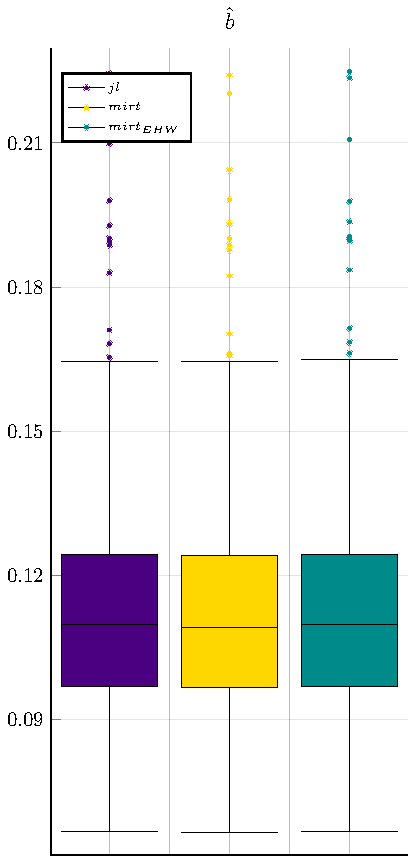
\includegraphics[width=.3\textwidth]{Figures/1a/RMSE_b.pdf} & 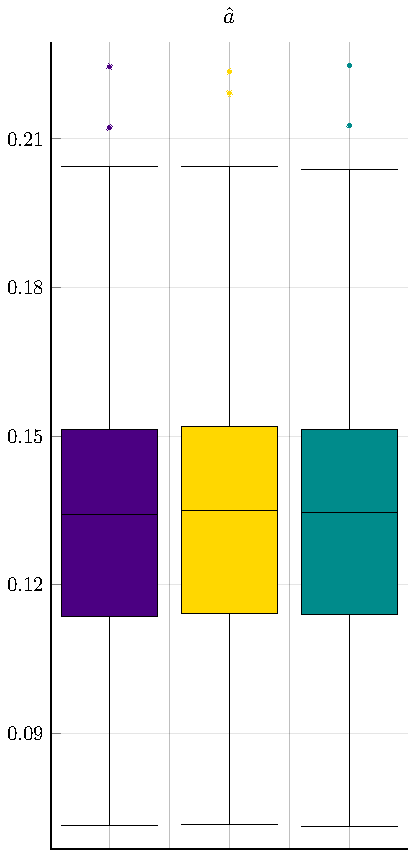
\includegraphics[width=.3\textwidth]{Figures/1a/RMSE_a.pdf} & 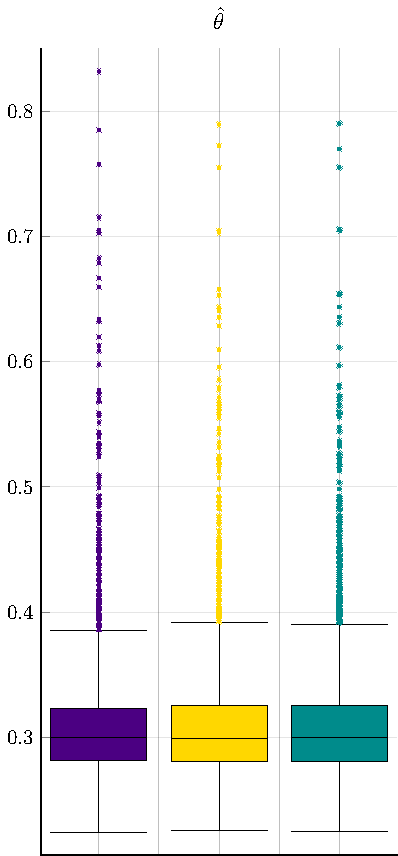
\includegraphics[width=.3\textwidth]{Figures/1a/RMSE_t.pdf}
	\end{tabular}
	\caption{Case 1a - Boxplots of RMSEs.}
	\label{fig:bpRMSE1a}
\end{figure}
\begin{figure}[H] 
	\centering \begin{tabular}[b]{c c c}
		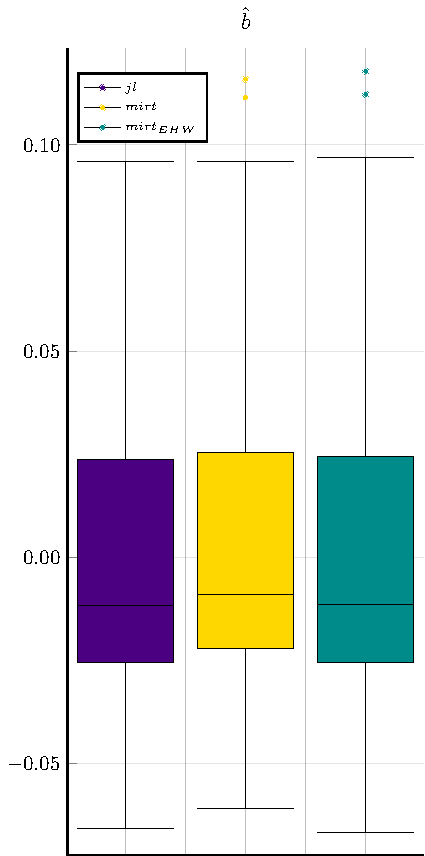
\includegraphics[width=.3\textwidth]{Figures/1a/BIAS_b.pdf} & 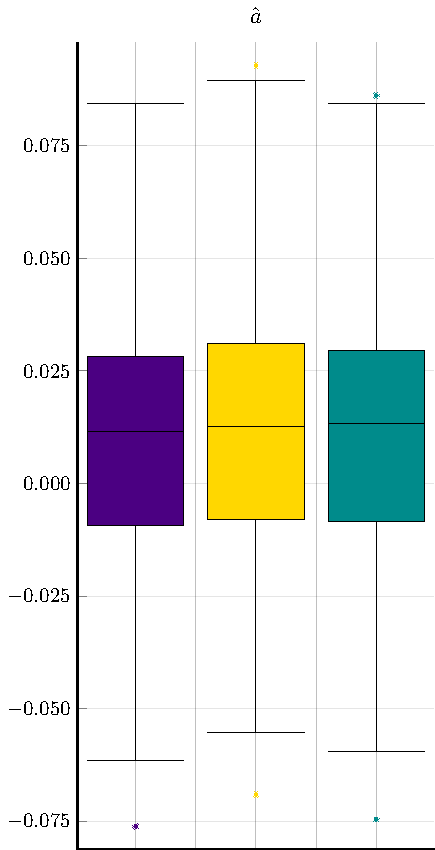
\includegraphics[width=.3\textwidth]{Figures/1a/BIAS_a.pdf} & 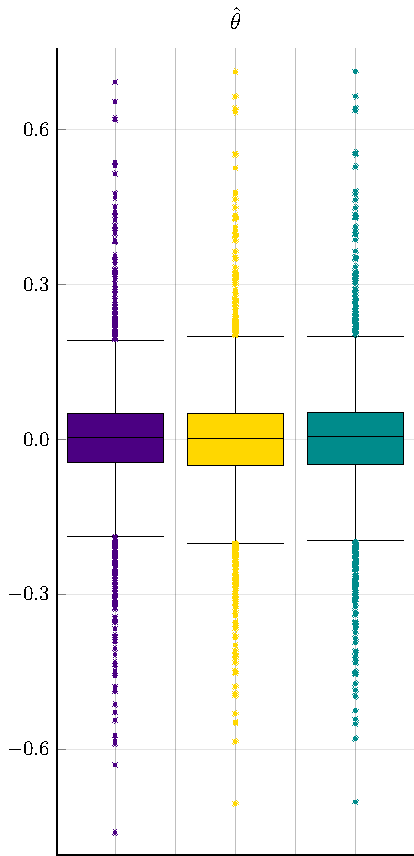
\includegraphics[width=.3\textwidth]{Figures/1a/BIAS_t.pdf}
	\end{tabular}
	\caption{Case 1a - Boxplots of BIASs.}
	\label{fig:bpBIAS1a}
\end{figure}
\begin{figure}[H] 
	\centering
	%\textbf{RMSEs of estimates with respect to the true values of item parameters and ability }\par\medskip
	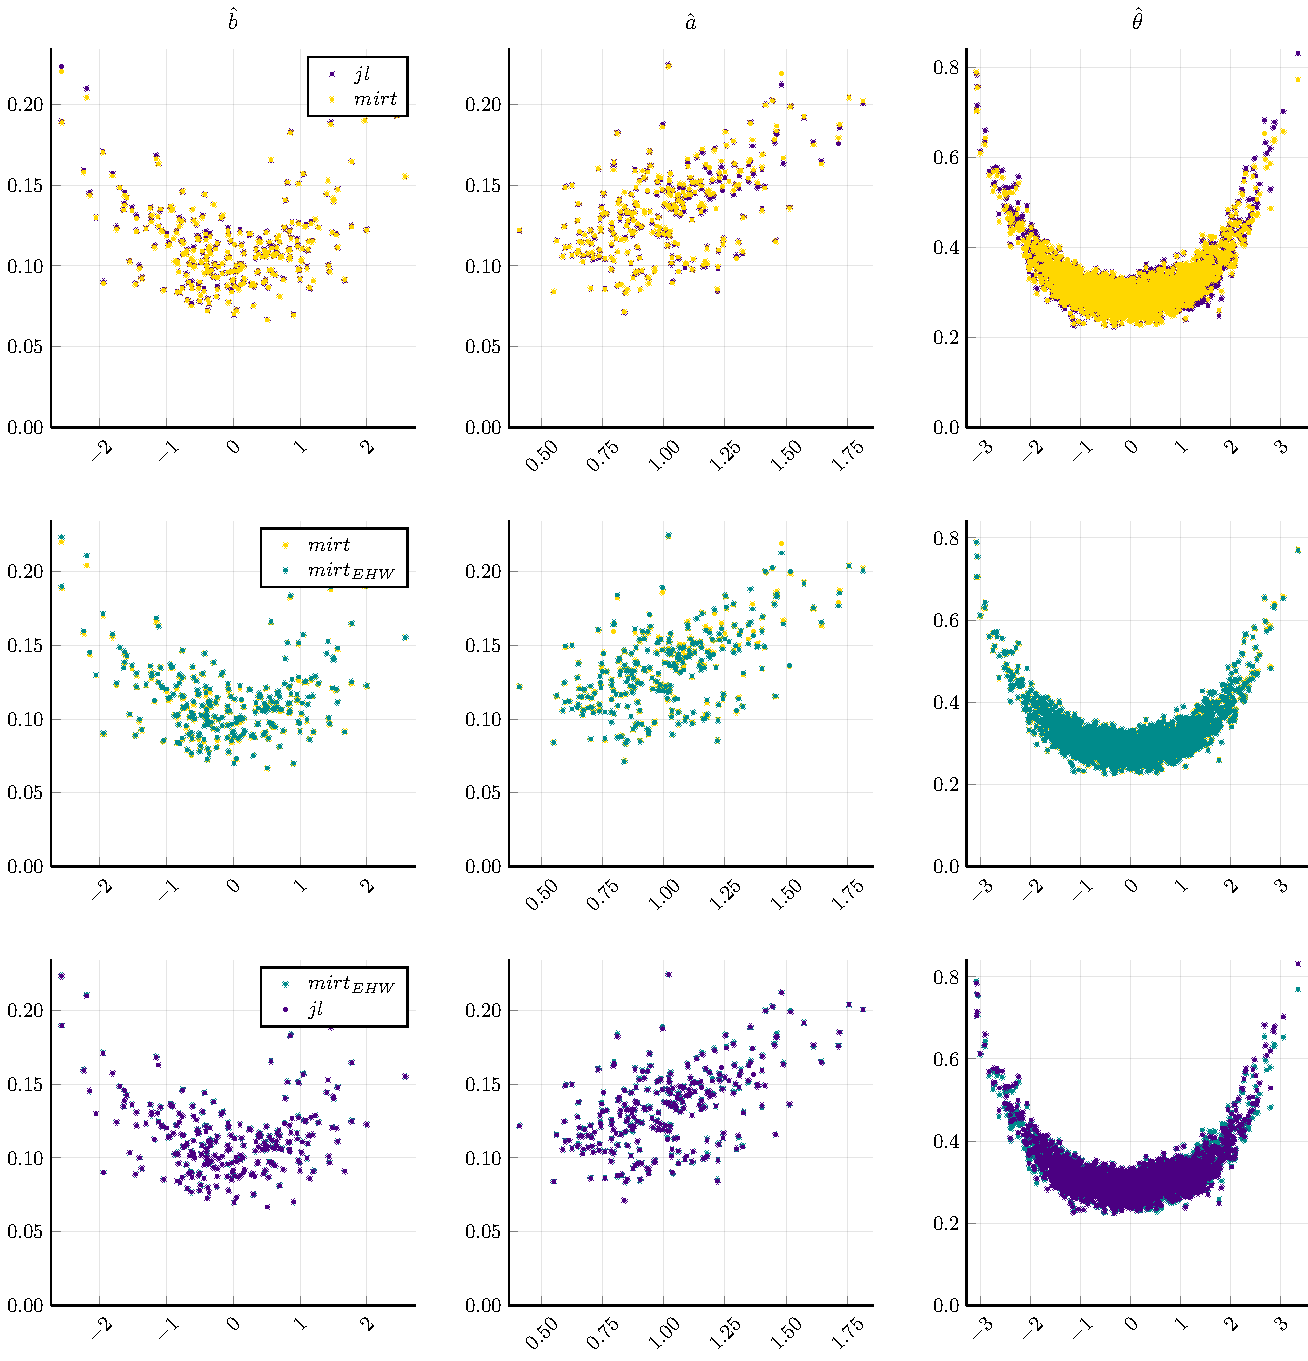
\includegraphics[width=\textwidth]{Figures/1a/RMSEscatter.pdf}
	\caption{Case 1a - Scatter plots of RMSEs.}
	\label{fig:spRMSE1a}
\end{figure}
\begin{figure}[H] 
	\centering
	%\textbf{BIASs of estimates with respect to the true values of item parameters and ability}\par\medskip
	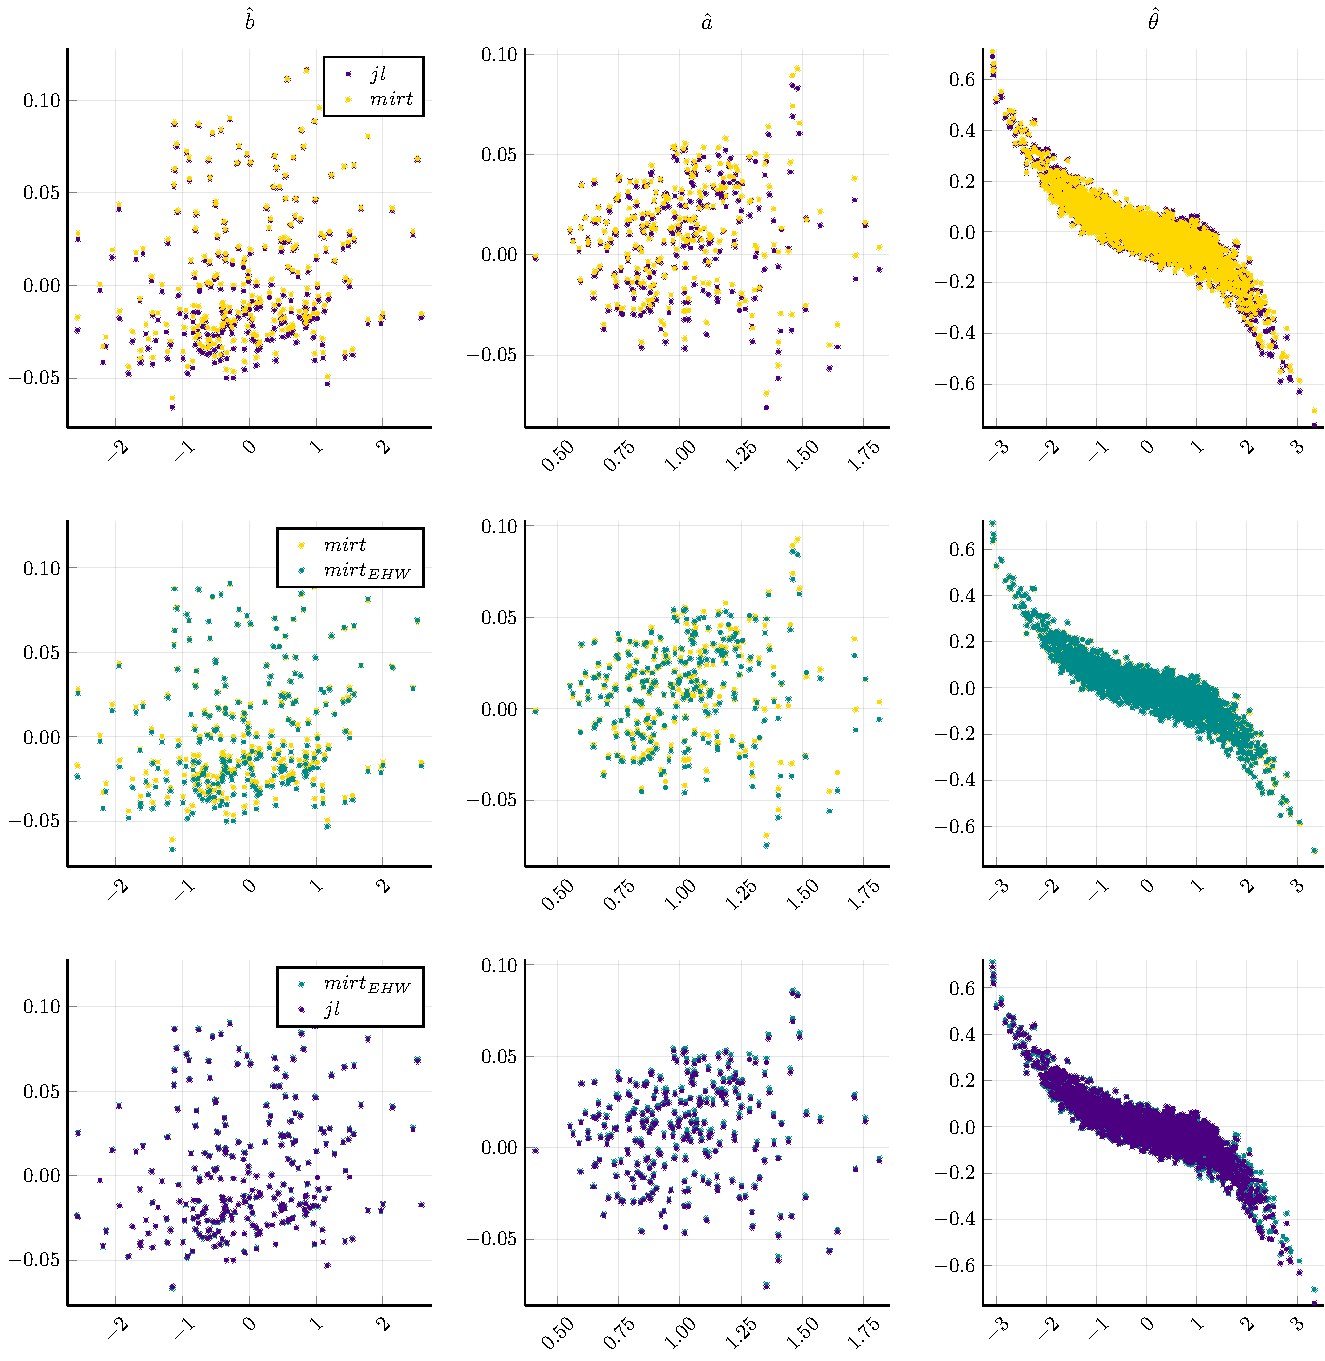
\includegraphics[width=\textwidth]{Figures/1a/BIASscatter.pdf}
	\caption{Case 1a - Scatter plots of BIASs }
	\label{fig:spBIAS1a}
\end{figure}
\subsection{Case 1b}
\begin{figure}[H] 
	\centering \begin{tabular}[b]{c c c}
		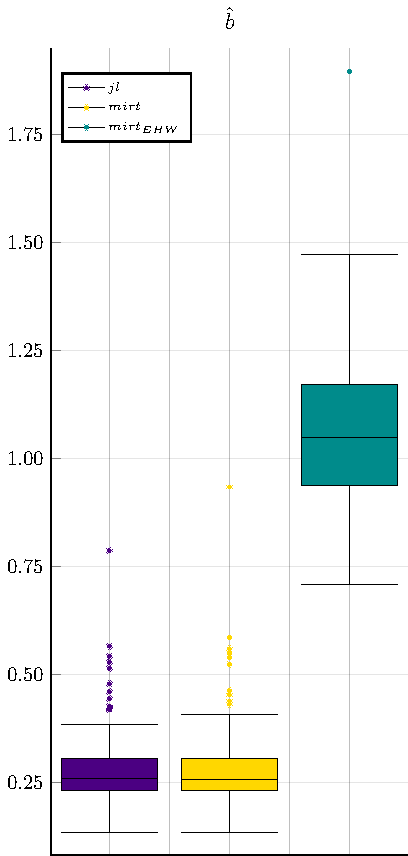
\includegraphics[width=.3\textwidth]{Figures/1b/RMSE_b.pdf} & 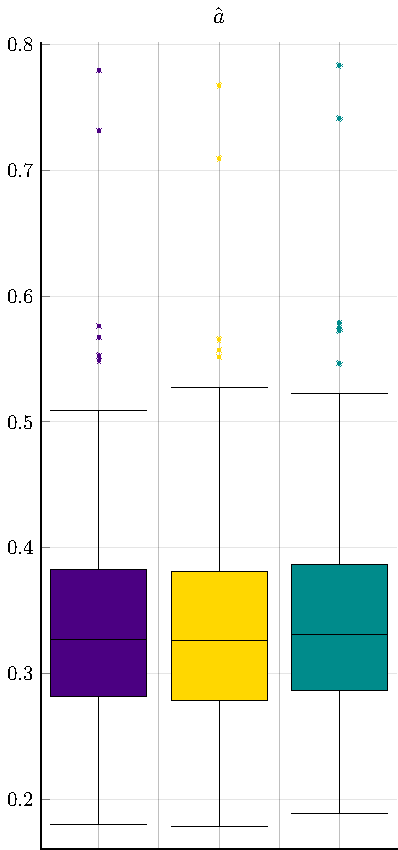
\includegraphics[width=.3\textwidth]{Figures/1b/RMSE_a.pdf} & 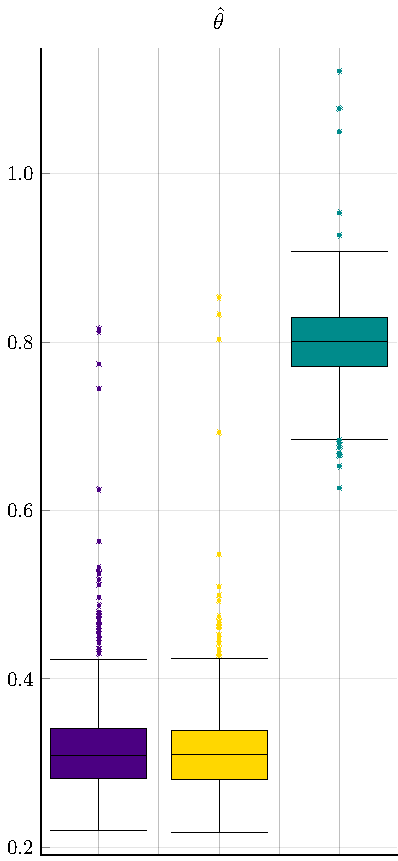
\includegraphics[width=.3\textwidth]{Figures/1b/RMSE_t.pdf}
	\end{tabular}
	\caption{Case 1b - Boxplots of RMSEs.}
	\label{fig:bpRMSE1b}
\end{figure}
\begin{figure}[H] 
	\centering \begin{tabular}[b]{c c c}
		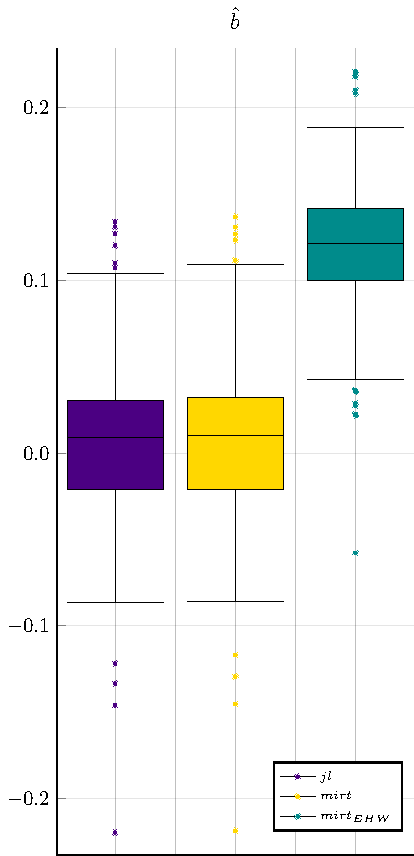
\includegraphics[width=.3\textwidth]{Figures/1b/BIAS_b.pdf} & 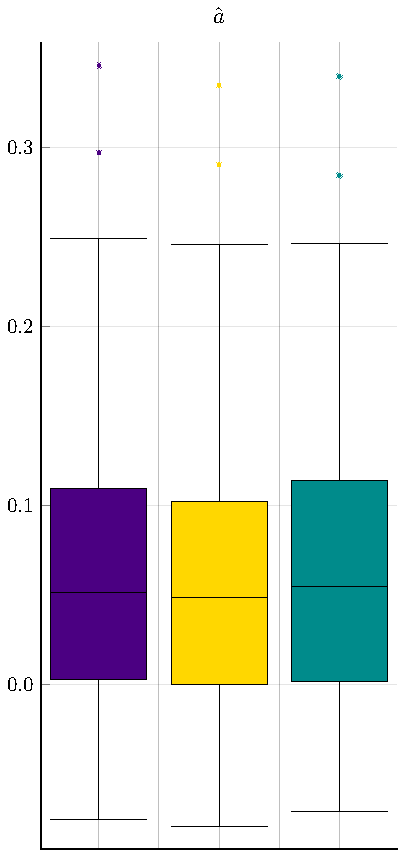
\includegraphics[width=.3\textwidth]{Figures/1b/BIAS_a.pdf} & 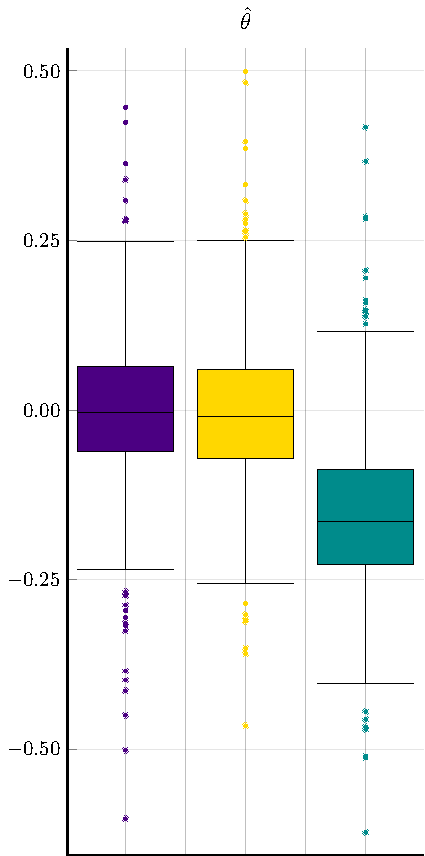
\includegraphics[width=.3\textwidth]{Figures/1b/BIAS_t.pdf}
	\end{tabular}
	\caption{Case 1b - Boxplots of BIASs.}
	\label{fig:bpBIAS1b}
\end{figure}
\begin{figure}[H] 
	\centering
	%\textbf{RMSEs of estimates with respect to the true values of item parameters and ability }\par\medskip
	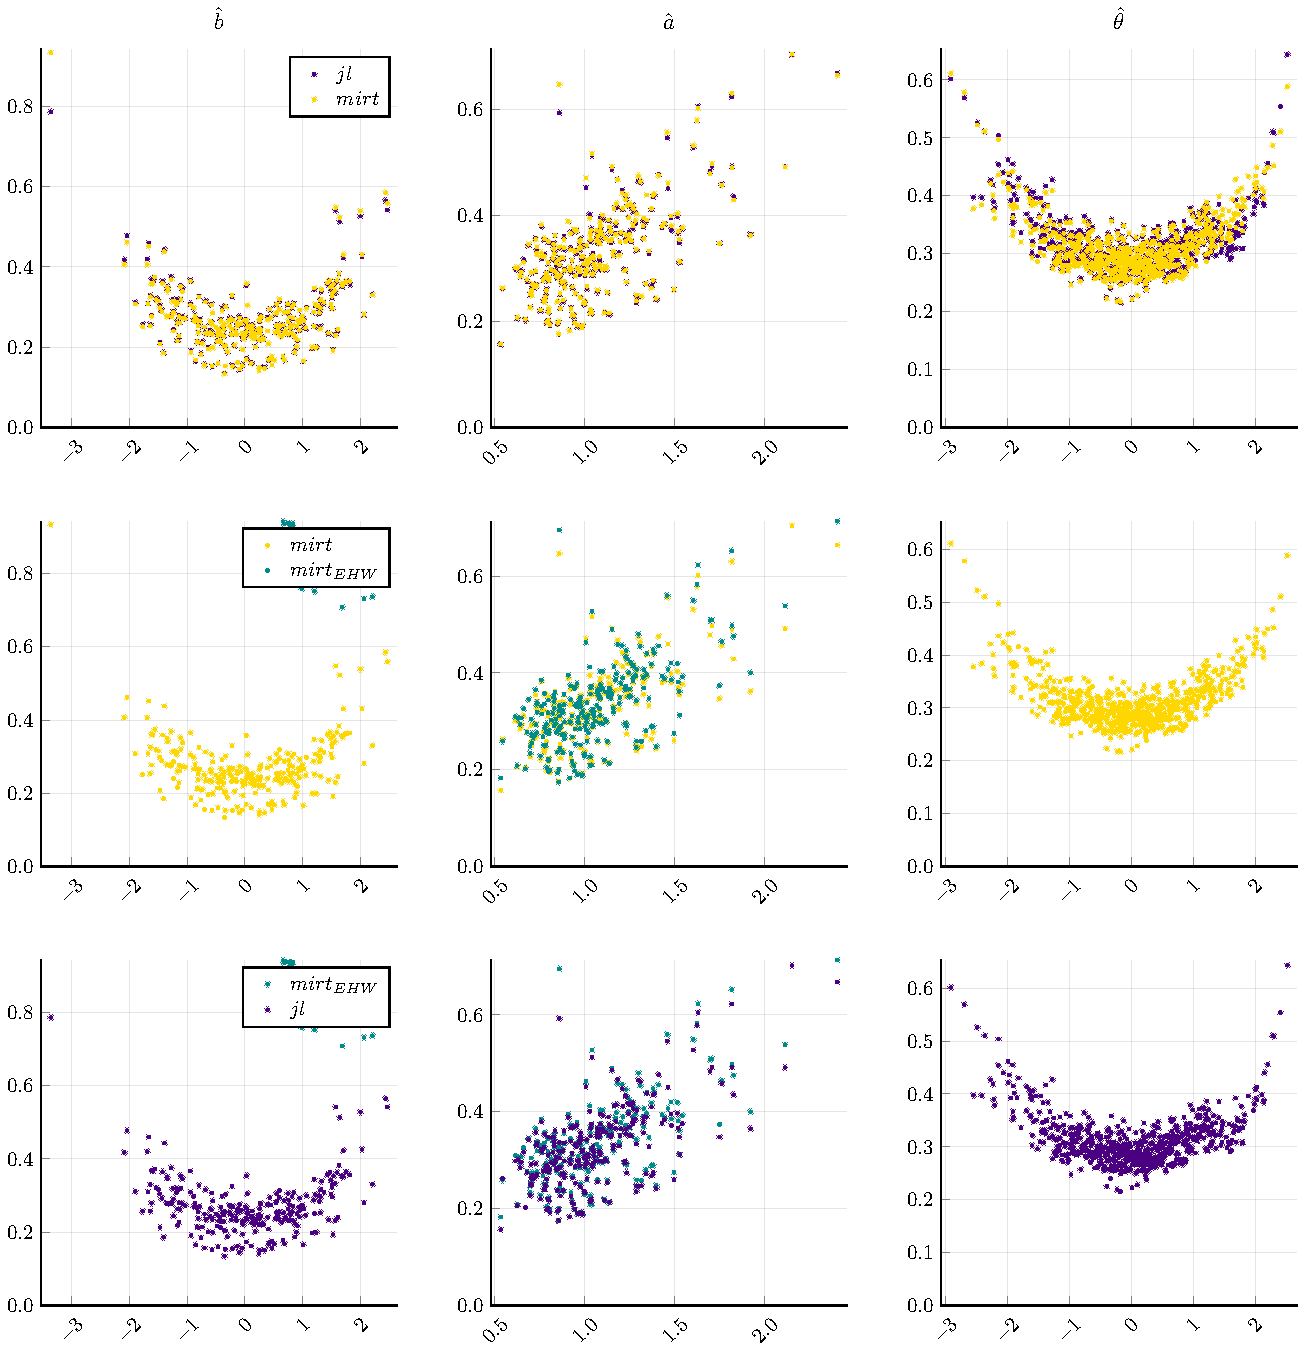
\includegraphics[width=\textwidth]{Figures/1b/RMSEscatter.pdf}
	\caption{Case 1b - Scatter plots of RMSEs.}
	\label{fig:spRMSE1b}
\end{figure}
\begin{figure}[H] 
	\centering
	%\textbf{BIASs of estimates with respect to the true values of item parameters and ability}\par\medskip
	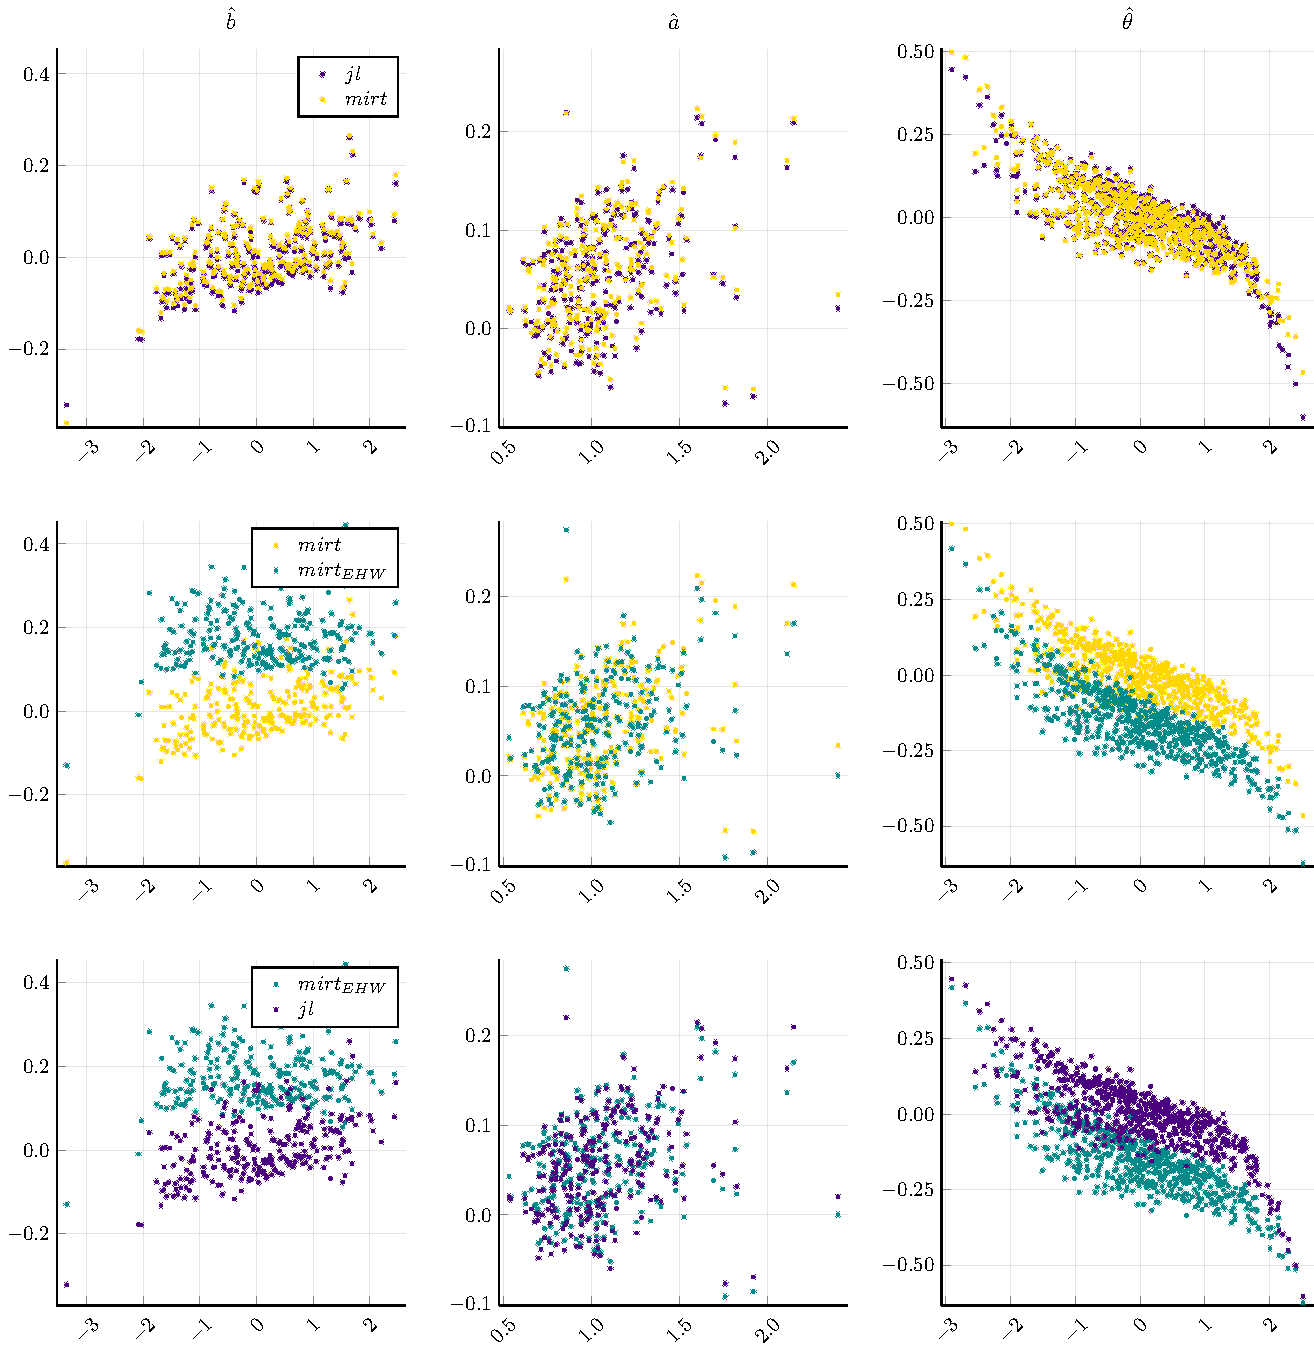
\includegraphics[width=\textwidth]{Figures/1b/BIASscatter.pdf}
	\caption{Case 1b - Scatter plots of BIASs }
	\label{fig:spBIAS1b}
\end{figure}
\subsection{Case 1c}
\begin{figure}[H] 
	\centering
	\begin{tabular}[b]{c c c}
		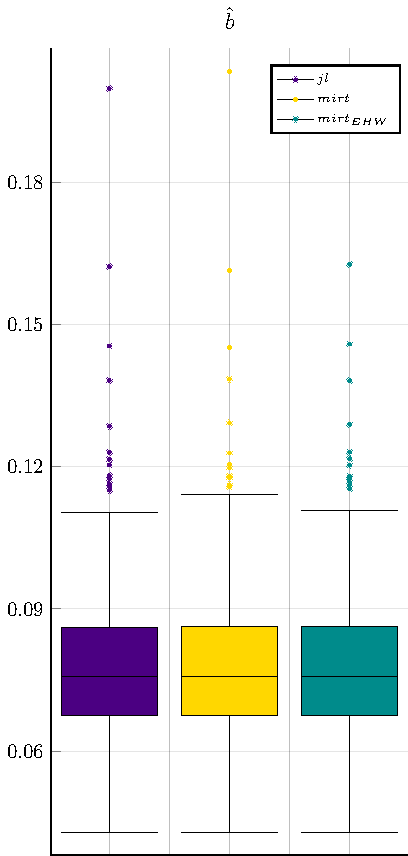
\includegraphics[width=.3\textwidth]{Figures/1c/RMSE_b.pdf} & 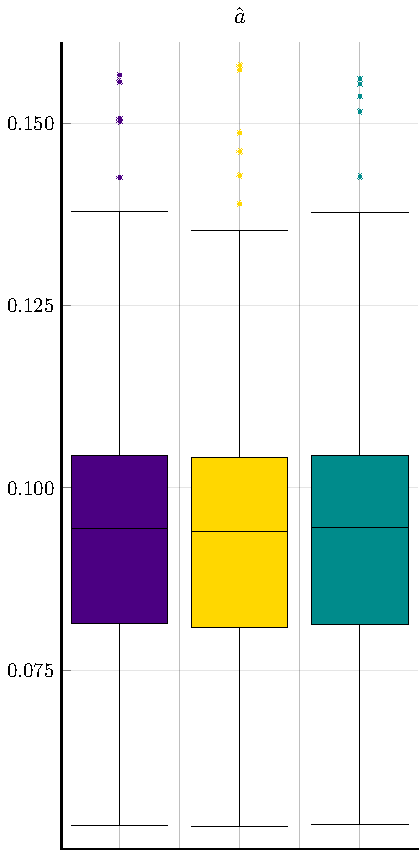
\includegraphics[width=.3\textwidth]{Figures/1c/RMSE_a.pdf} & 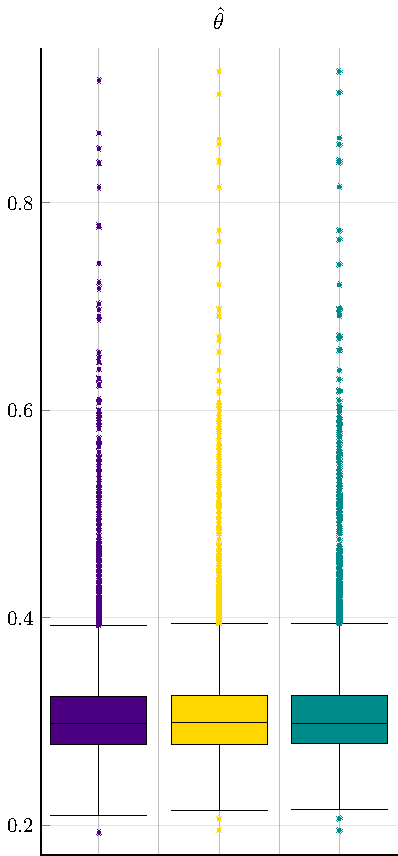
\includegraphics[width=.3\textwidth]{Figures/1c/RMSE_t.pdf}
	\end{tabular}
	\caption{Case 1c - Boxplots of RMSEs.}
	\label{fig:bpRMSE1c}
\end{figure}
\begin{figure}[H] 
	
	\centering
	\begin{tabular}[b]{c c c}
		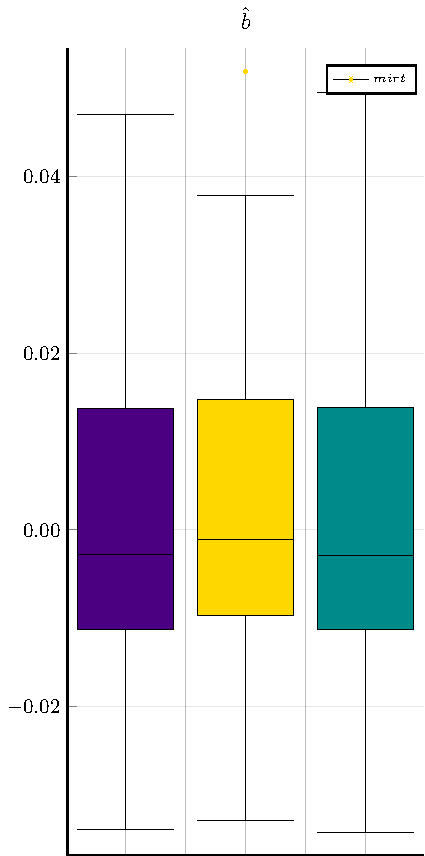
\includegraphics[width=.3\textwidth]{Figures/1c/BIAS_b.pdf} & 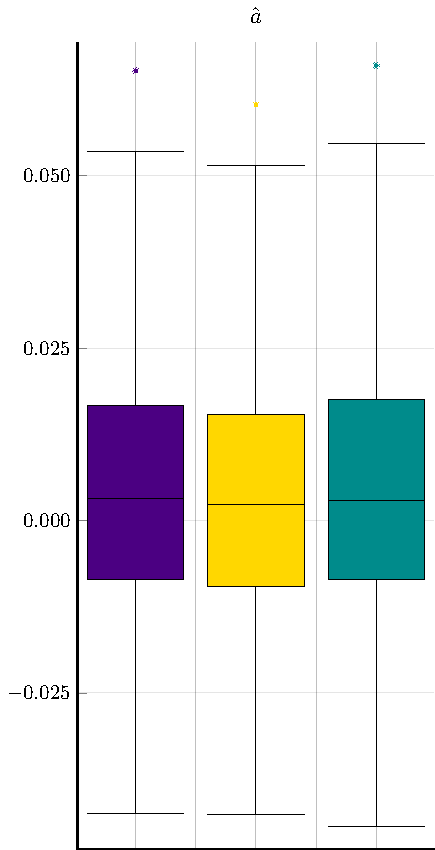
\includegraphics[width=.3\textwidth]{Figures/1c/BIAS_a.pdf} & 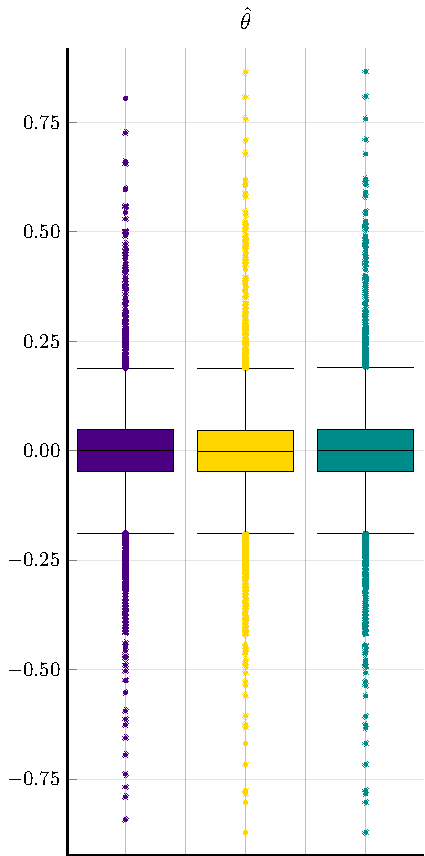
\includegraphics[width=.3\textwidth]{Figures/1c/BIAS_t.pdf}
	\end{tabular}
	\caption{Case 1c - Boxplots of BIASs.}
	\label{fig:bpBIAS1c}
\end{figure}
\begin{figure}[H] 
	\centering
	%\textbf{RMSEs of estimates with respect to the true values of item parameters and ability }\par\medskip
	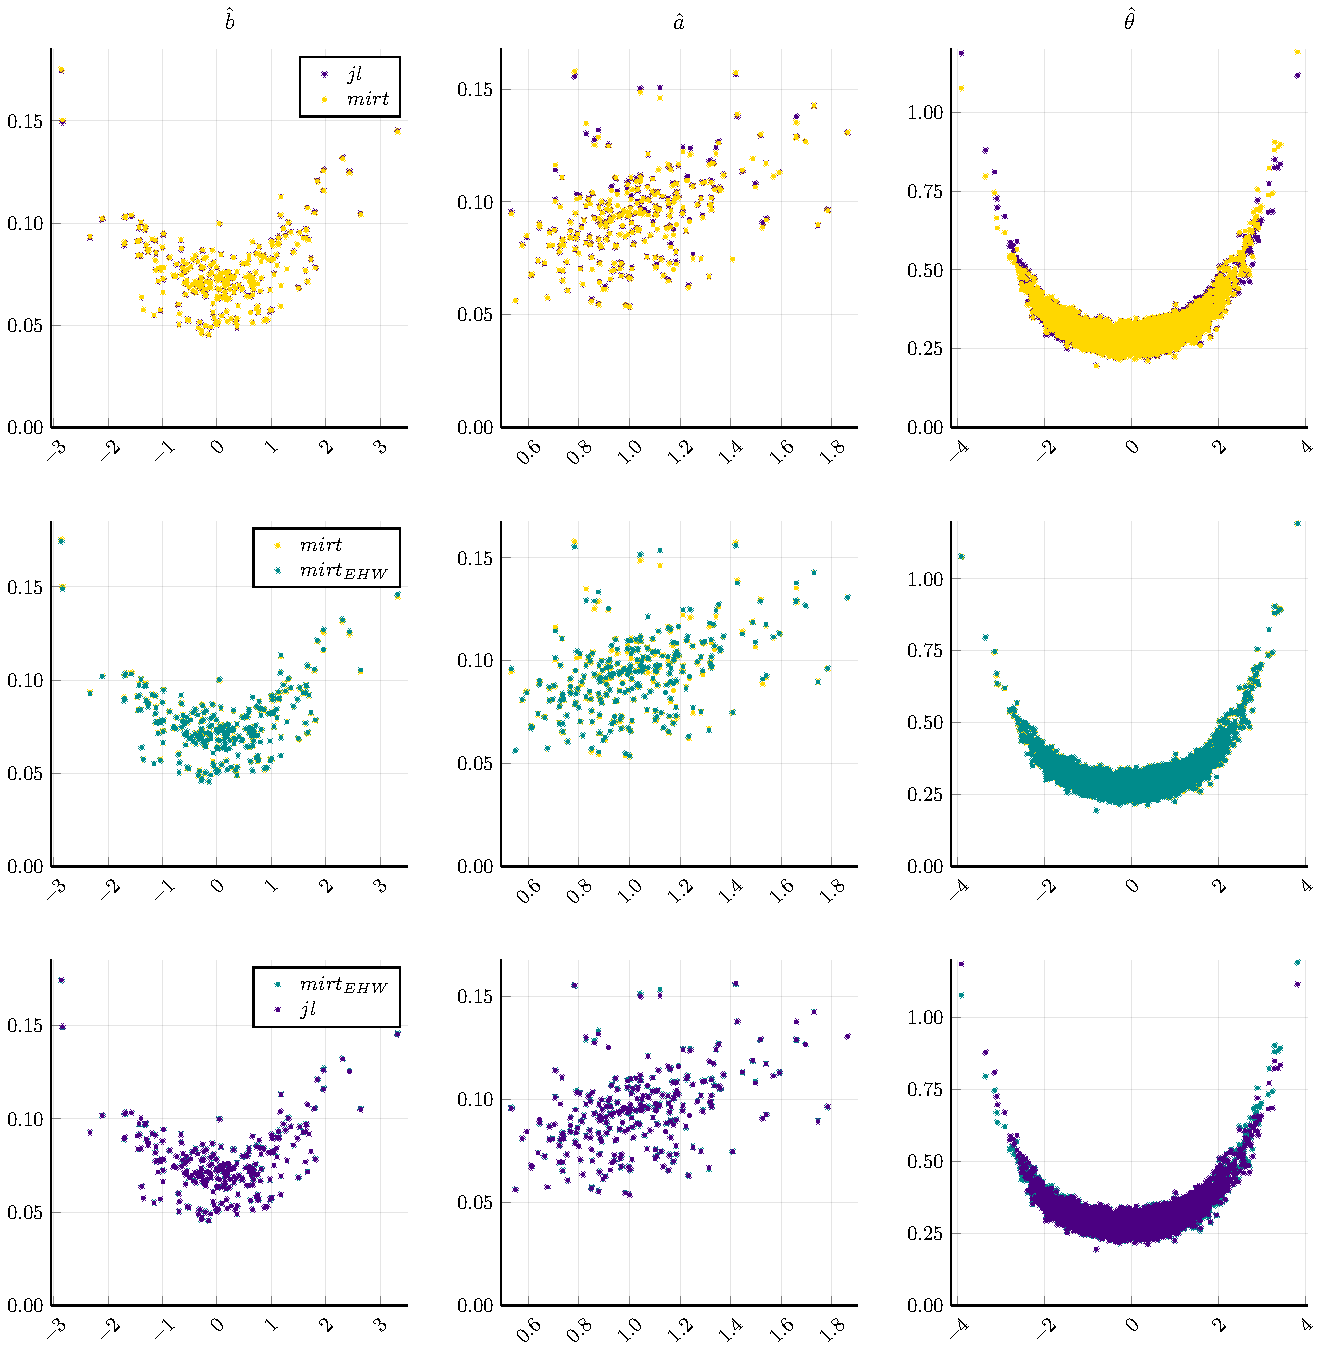
\includegraphics[width=\textwidth]{Figures/1c/RMSEscatter.pdf}
	\caption{Case 1c - Scatter plots of RMSEs.}
	\label{fig:spRMSE1c}
\end{figure}
\begin{figure}[H] 
	\centering
	%\textbf{BIASs of estimates with respect to the true values of item parameters and ability}\par\medskip
	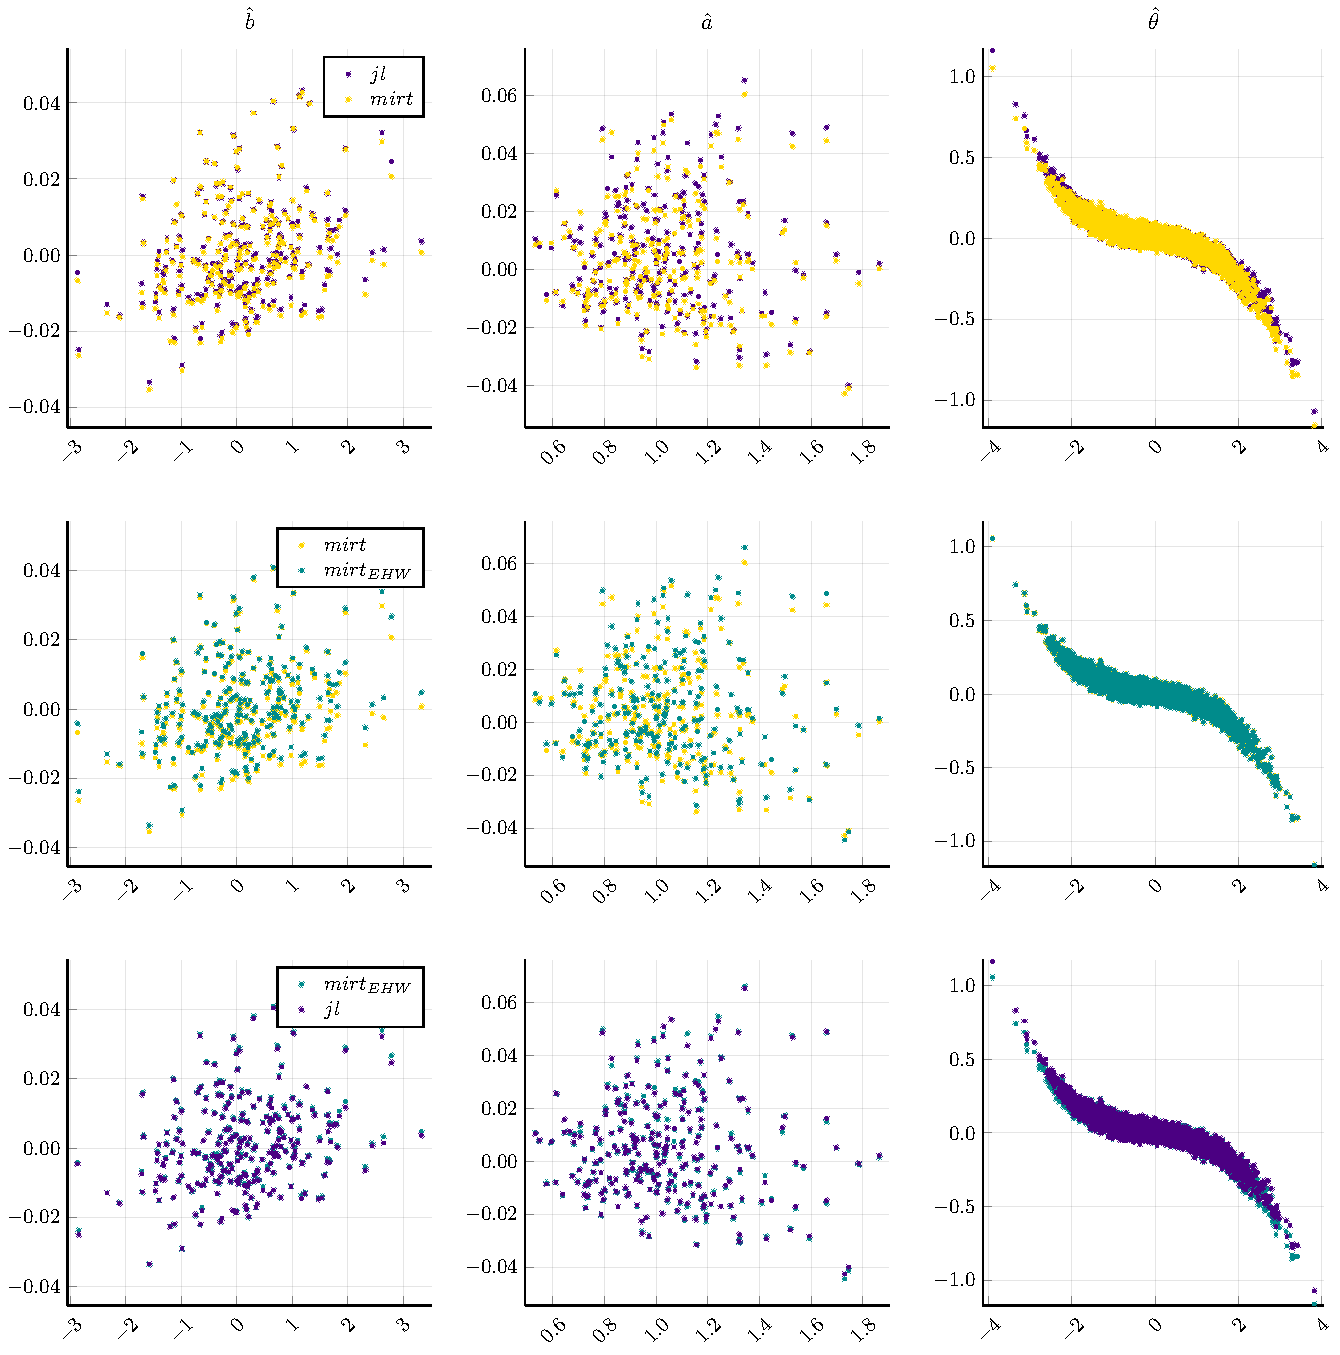
\includegraphics[width=\textwidth]{Figures/1c/BIASscatter.pdf}
	\caption{Case 1c - Scatter plots of BIASs }
	\label{fig:spBIAS1c}
\end{figure}
\subsection{Case 2a}
\begin{figure}[H] 
	\centering
	\begin{tabular}[b]{c c c}
		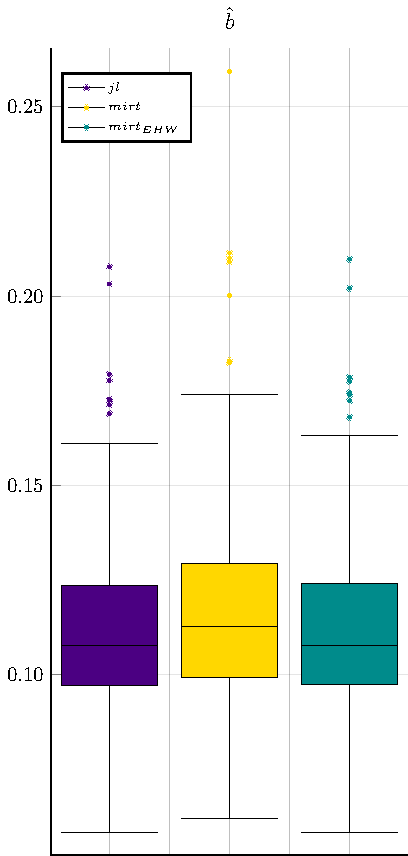
\includegraphics[width=.3\textwidth]{Figures/2a/RMSE_b.pdf} & 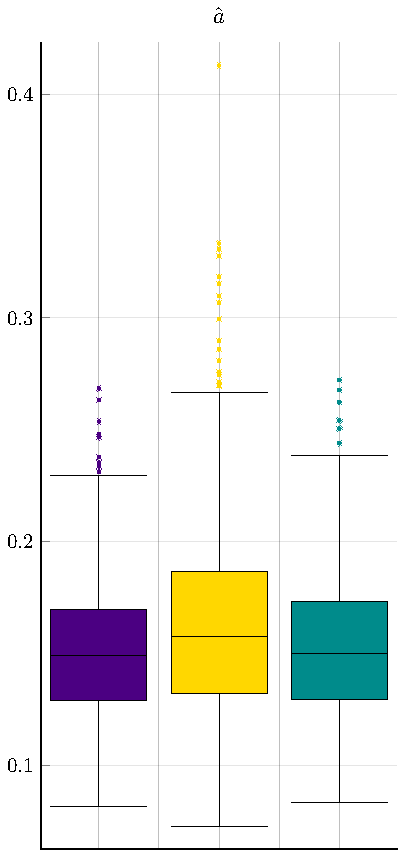
\includegraphics[width=.3\textwidth]{Figures/2a/RMSE_a.pdf} & 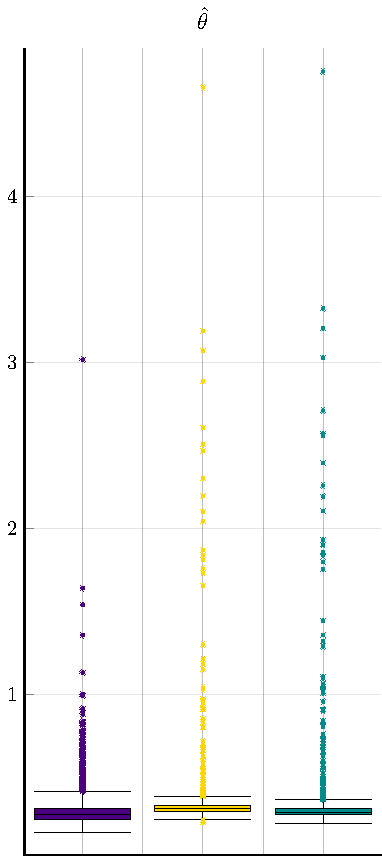
\includegraphics[width=.3\textwidth]{Figures/2a/RMSE_t.pdf}
	\end{tabular}
	\caption{Case 2a - Boxplots of RMSEs.}
	\label{fig:bpRMSE2a}
\end{figure}
\begin{figure}[H] 
	\centering
	\begin{tabular}[b]{c c c}
		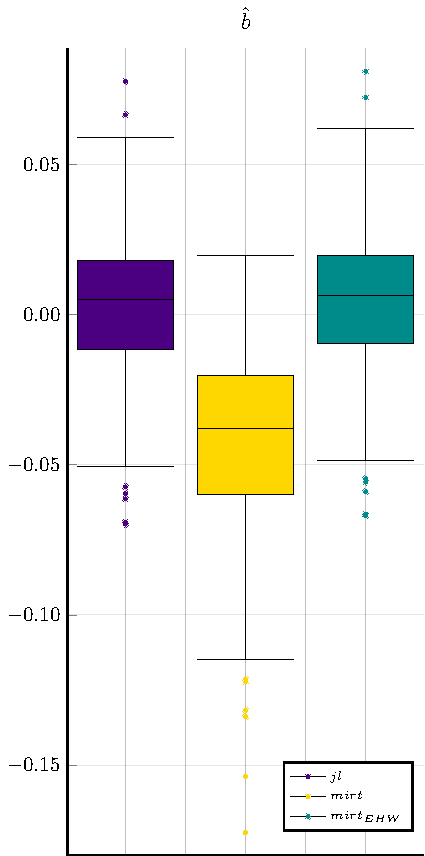
\includegraphics[width=.3\textwidth]{Figures/2a/BIAS_b.pdf} & 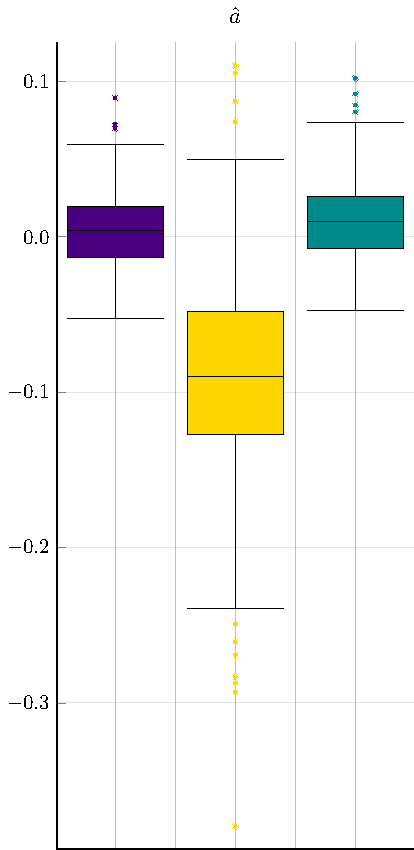
\includegraphics[width=.3\textwidth]{Figures/2a/BIAS_a.pdf} & 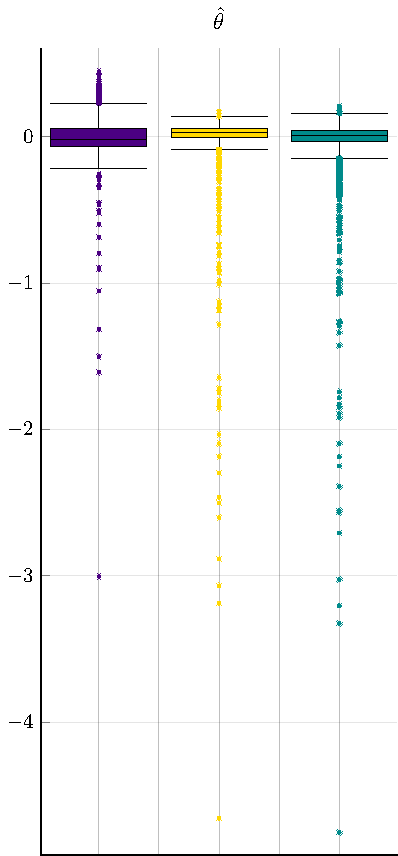
\includegraphics[width=.3\textwidth]{Figures/2a/BIAS_t.pdf}
	\end{tabular}
	\caption{Case 2a - Boxplots of BIASs.}
	\label{fig:bpBIAS2a}
\end{figure}
\begin{figure}[H] 
	\centering
	%\textbf{RMSEs of estimates with respect to the true values of item parameters and ability }\par\medskip
	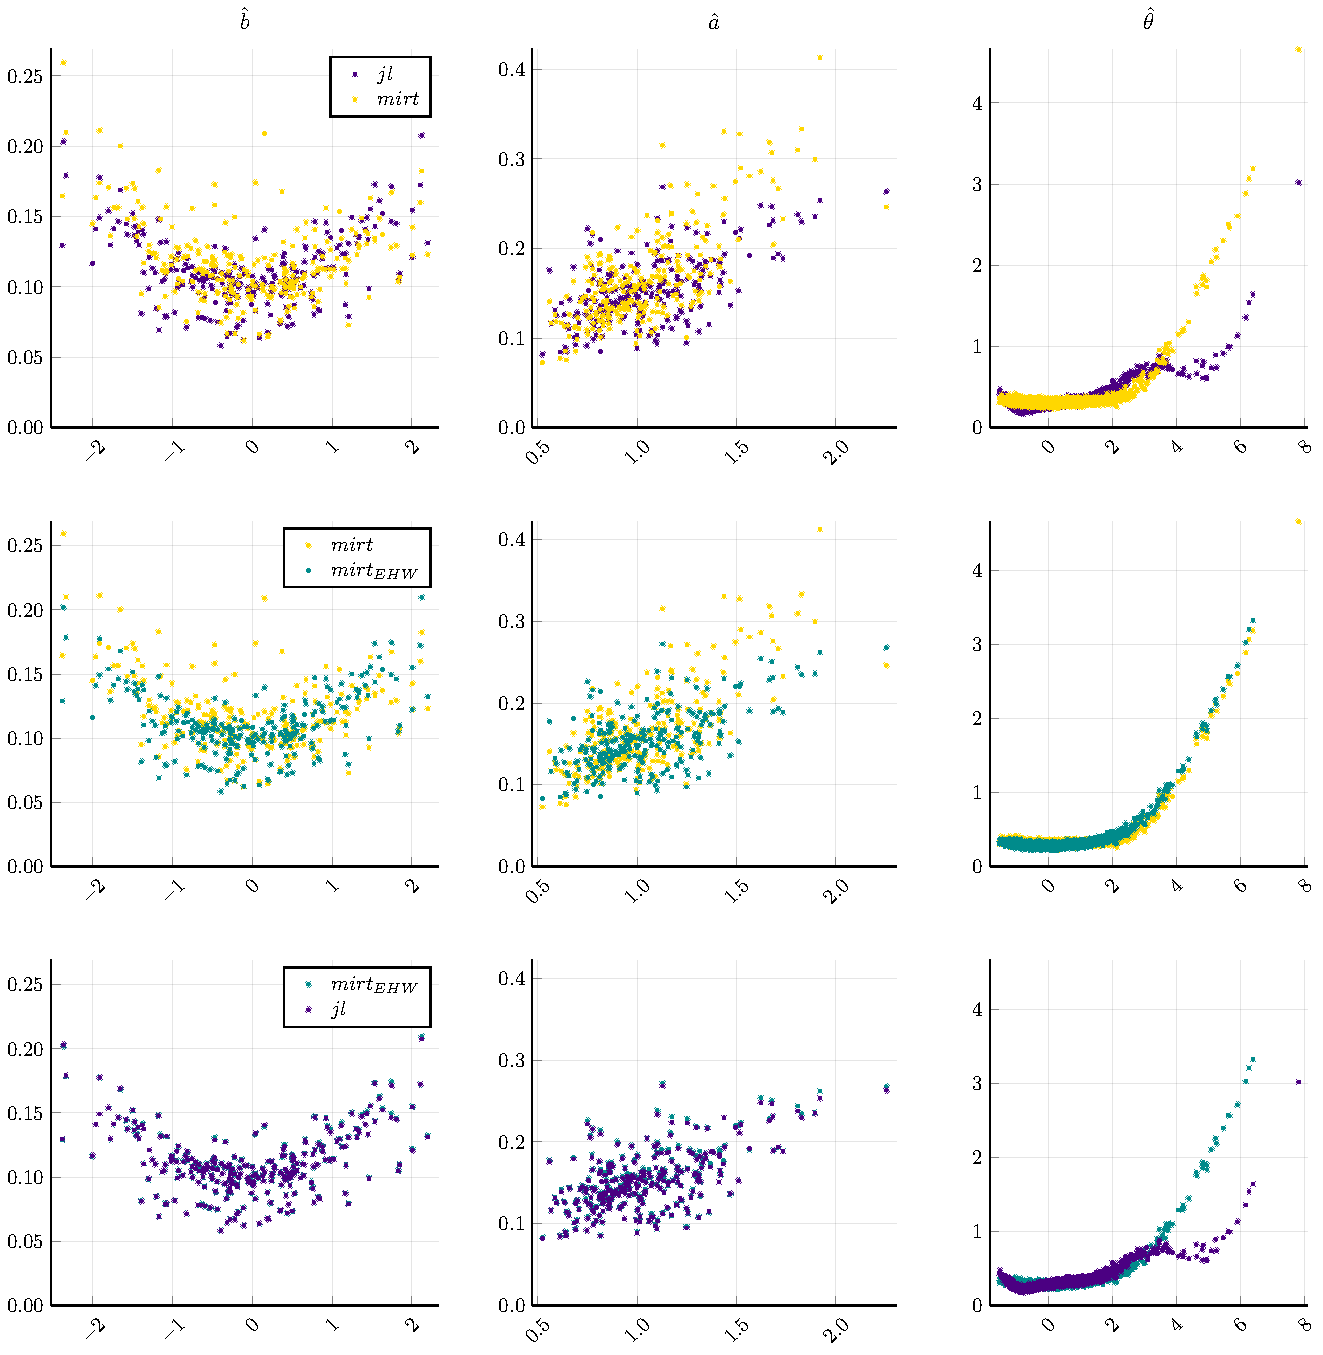
\includegraphics[width=\textwidth]{Figures/2a/RMSEscatter.pdf}
	\caption{Case 2a - Scatter plots of RMSEs.}
	\label{fig:spRMSE2a}
\end{figure}
\begin{figure}[H] 
	\centering
	%\textbf{BIASs of estimates with respect to the true values of item parameters and ability}\par\medskip
	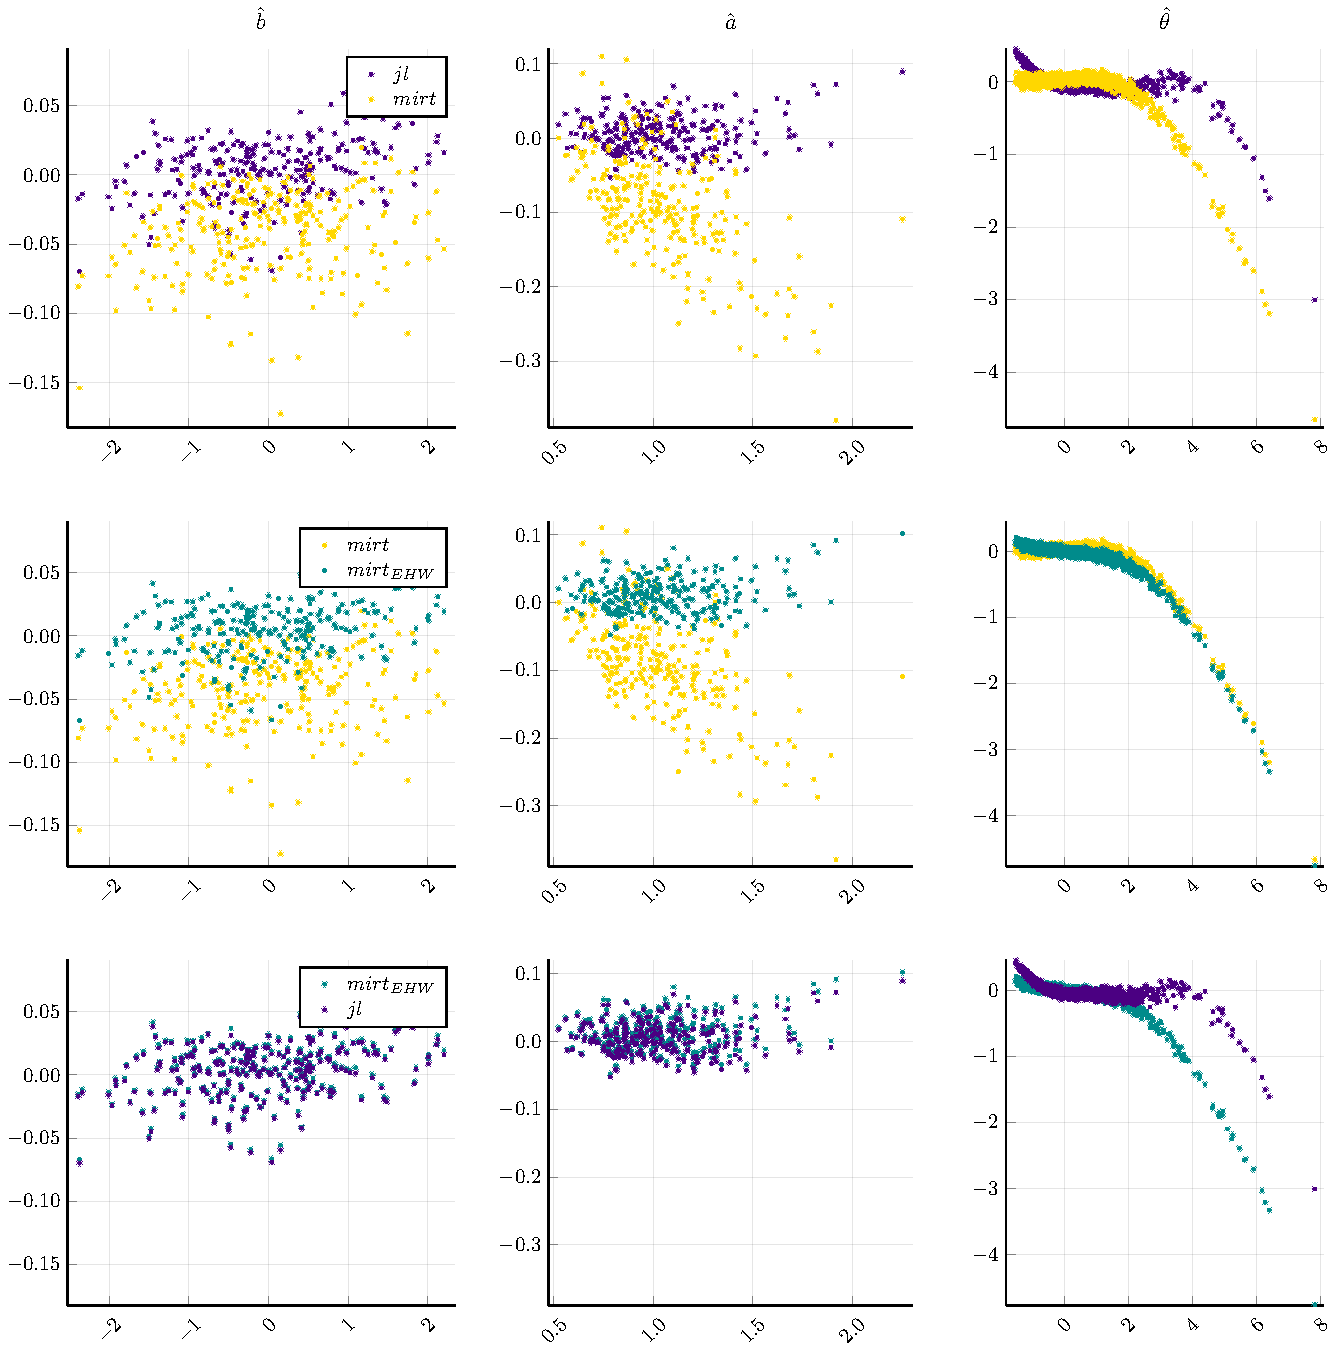
\includegraphics[width=\textwidth]{Figures/2a/BIASscatter.pdf}
	\caption{Case 2a - Scatter plots of BIASs }
	\label{fig:spBIAS2a}
\end{figure}
\subsection{Case 2b}
\begin{figure}[H] 
	
	\centering
	\begin{tabular}[b]{c c c}
		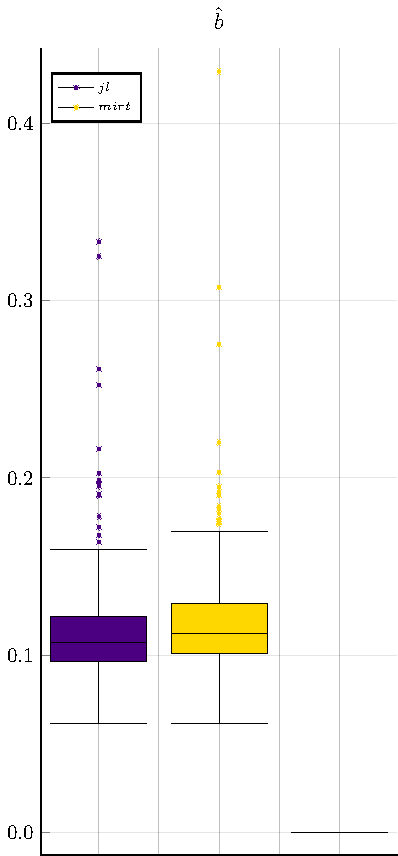
\includegraphics[width=.3\textwidth]{Figures/2b/RMSE_b.pdf} & 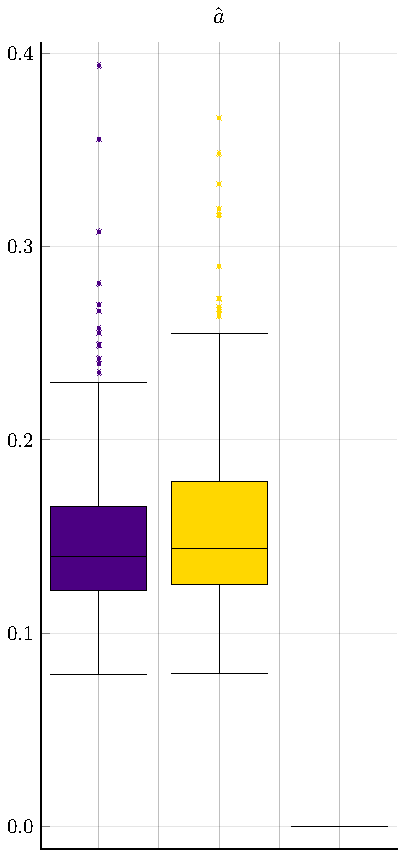
\includegraphics[width=.3\textwidth]{Figures/2b/RMSE_a.pdf} & 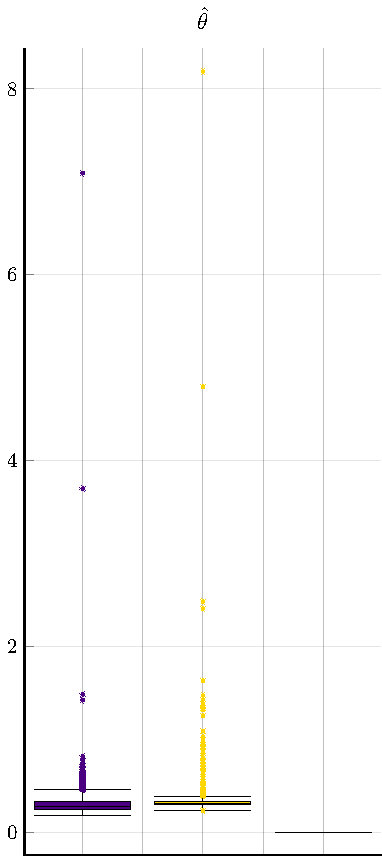
\includegraphics[width=.3\textwidth]{Figures/2b/RMSE_t.pdf}
	\end{tabular}
	\caption{Case 2b - Boxplots of RMSEs.}
	\label{fig:bpRMSE2b}
\end{figure}
\begin{figure}[H] 
	
	\centering \begin{tabular}[b]{c c c}
		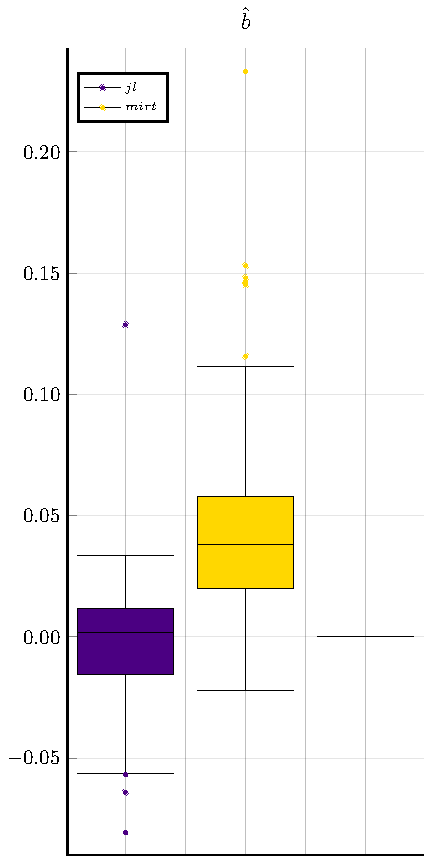
\includegraphics[width=.3\textwidth]{Figures/2b/BIAS_b.pdf} & 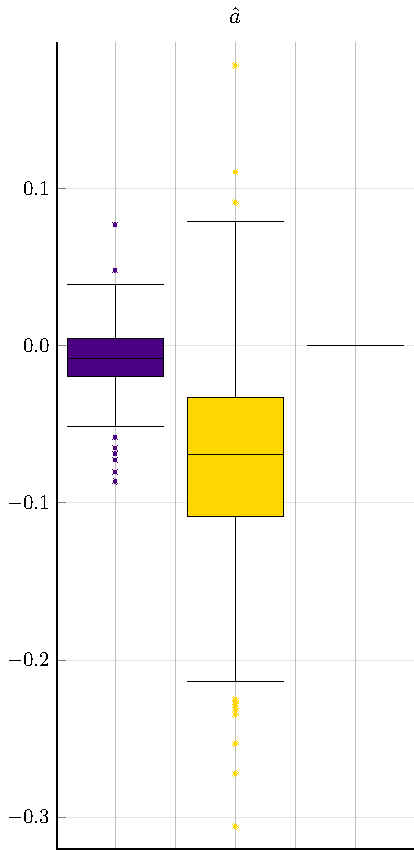
\includegraphics[width=.3\textwidth]{Figures/2b/BIAS_a.pdf} & 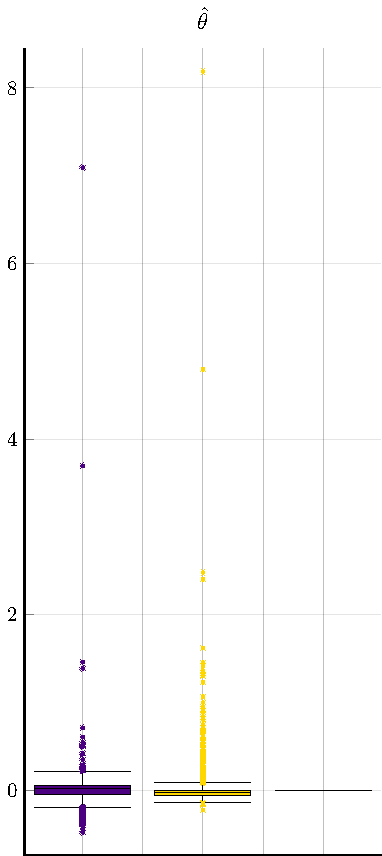
\includegraphics[width=.3\textwidth]{Figures/2b/BIAS_t.pdf}
	\end{tabular}
	\caption{Case 2b - Boxplots of BIASs.}
	\label{fig:bpBIAS2b}
\end{figure}
\begin{figure}[H] 
	\centering
	%\textbf{RMSEs of estimates with respect to the true values of item parameters and ability }\par\medskip
	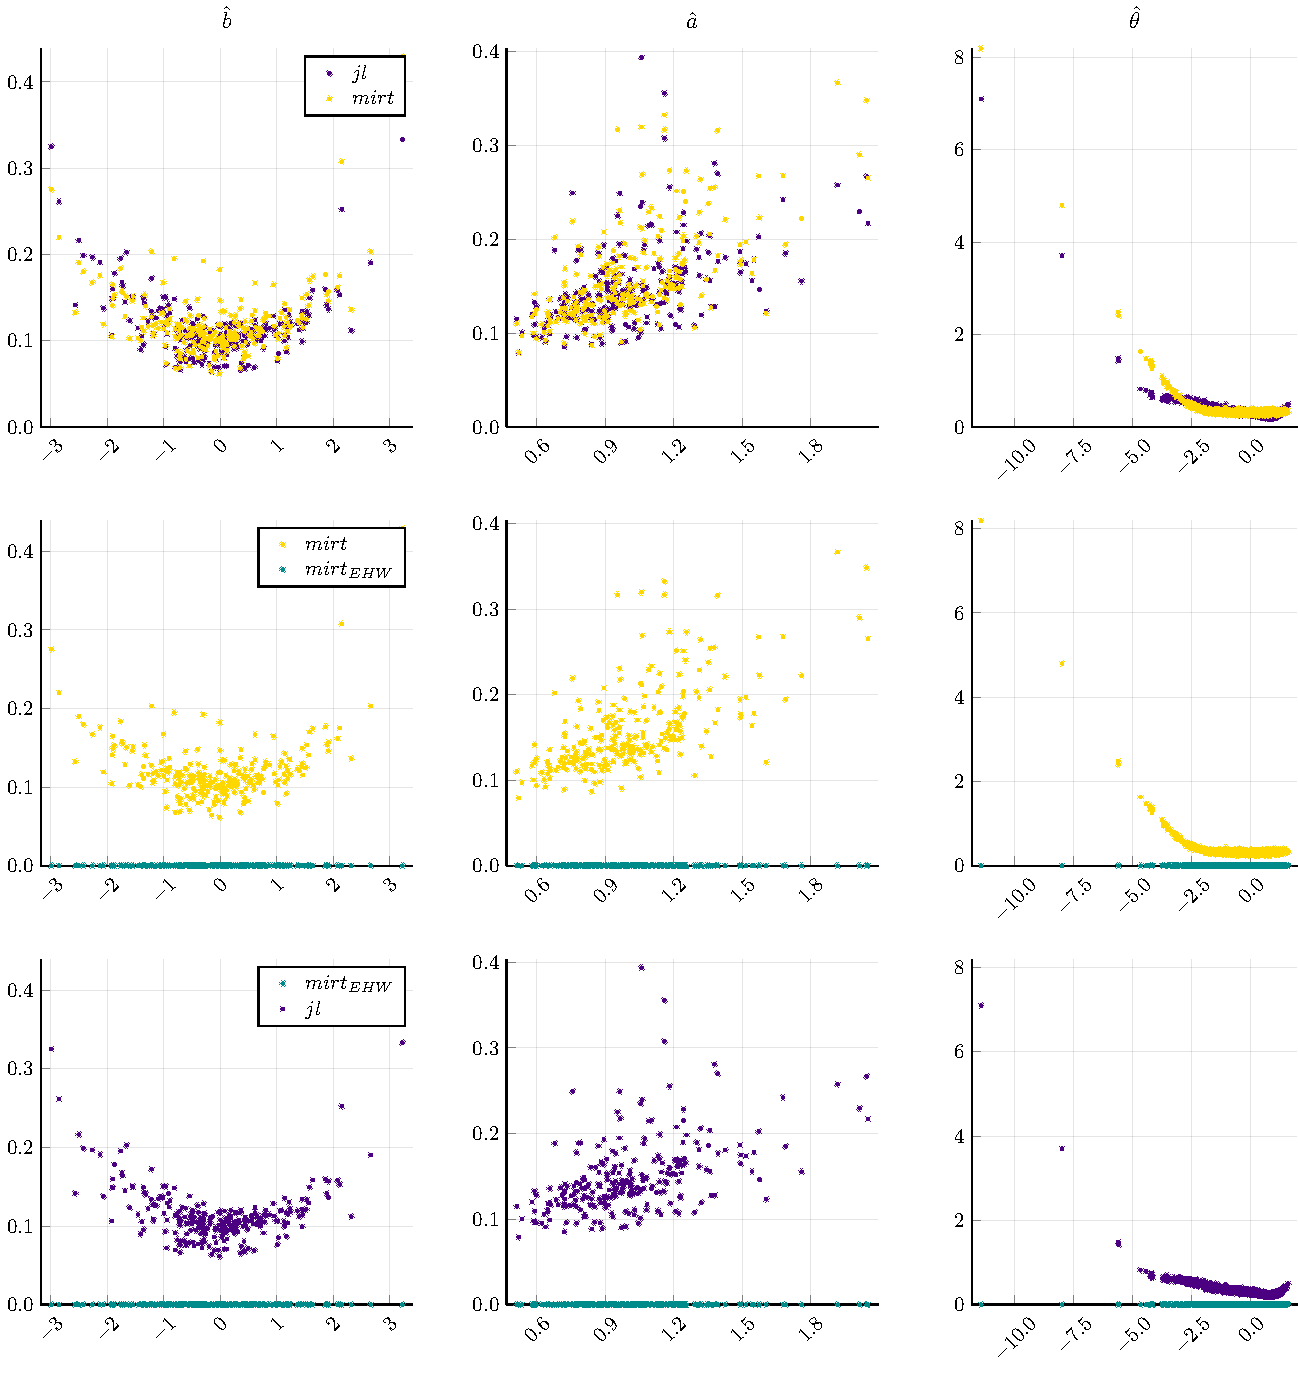
\includegraphics[width=\textwidth]{Figures/2b/RMSEscatter.pdf}
	\caption{Case 2b - Scatter plots of RMSEs.}
	\label{fig:spRMSE2b}
\end{figure}
\begin{figure}[H] 
	\centering
	%\textbf{BIASs of estimates with respect to the true values of item parameters and ability}\par\medskip
	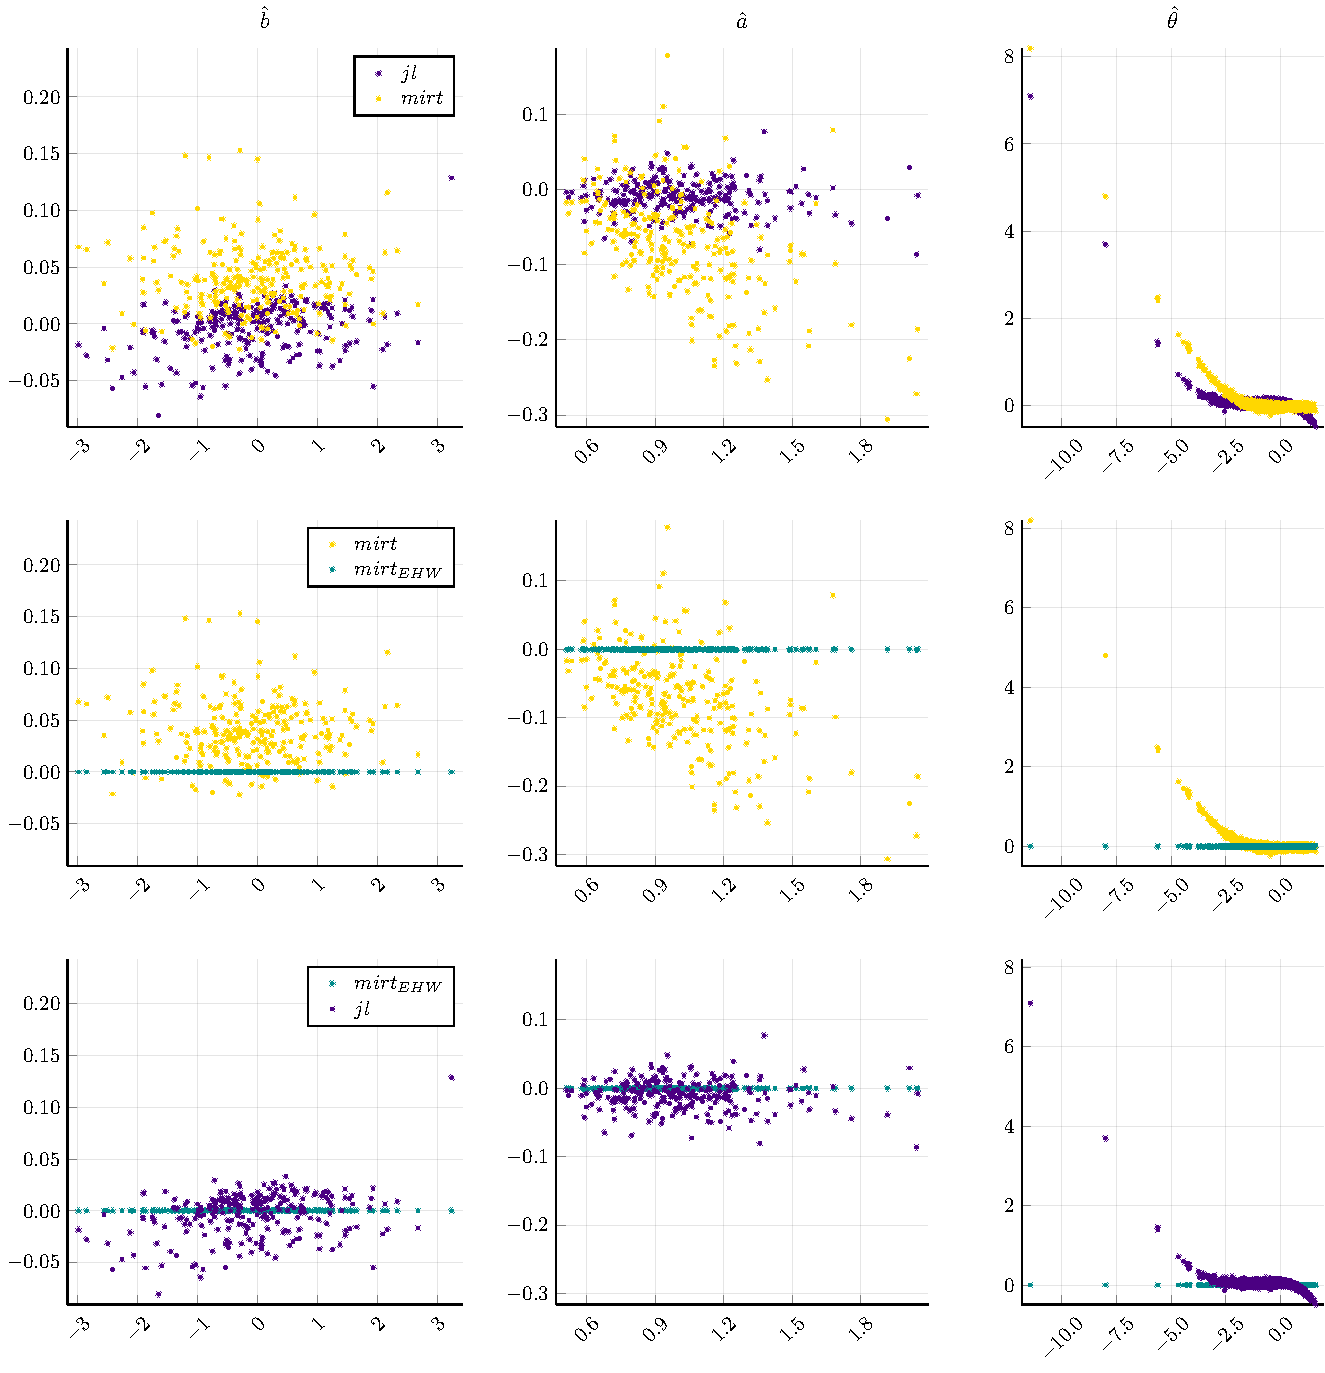
\includegraphics[width=\textwidth]{Figures/2b/BIASscatter.pdf}
	\caption{Case 2b - Scatter plots of BIASs }
	\label{fig:spBIAS2b}
\end{figure}
\subsection{Case 3}
\begin{figure}[H] 
	
	\centering
	\begin{tabular}[b]{c c c}
		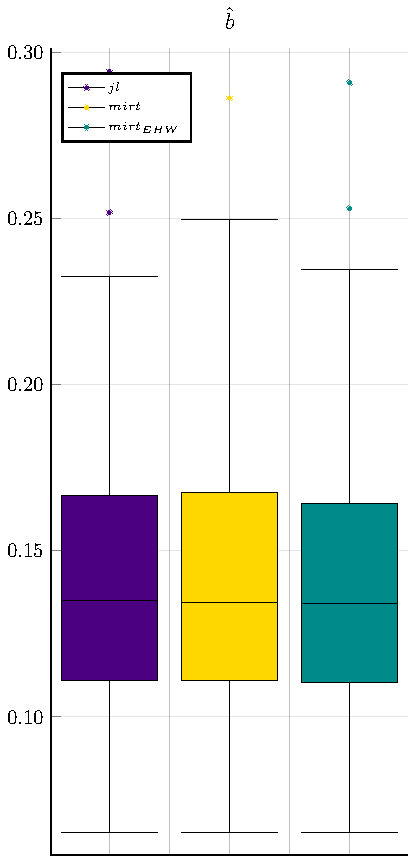
\includegraphics[width=.30\textwidth]{Figures/3/RMSE_b.pdf} & 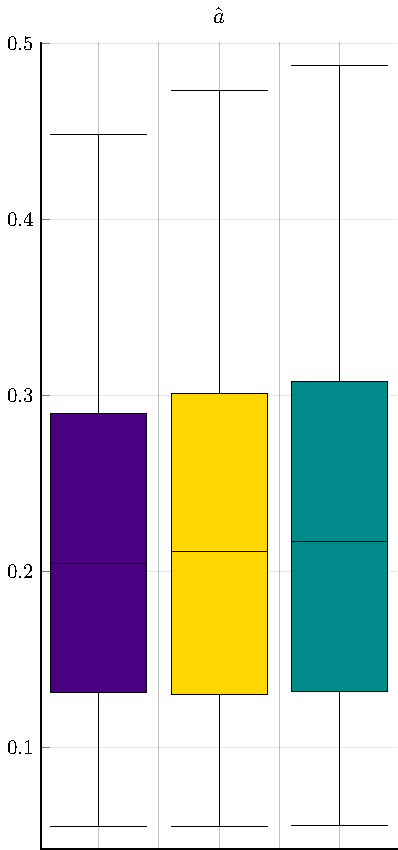
\includegraphics[width=.3\textwidth]{Figures/3/RMSE_a.pdf} & 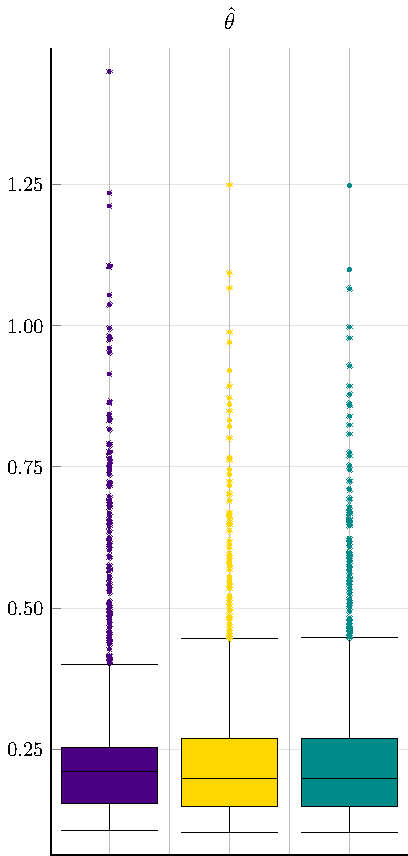
\includegraphics[width=.3\textwidth]{Figures/3/RMSE_t.pdf}
	\end{tabular}
	\caption{Case 3 - Boxplots of RMSEs.}
	\label{fig:bpRMSE3}
\end{figure}
\begin{figure}[H] 
	
	\centering
	\begin{tabular}[b]{c c c}
		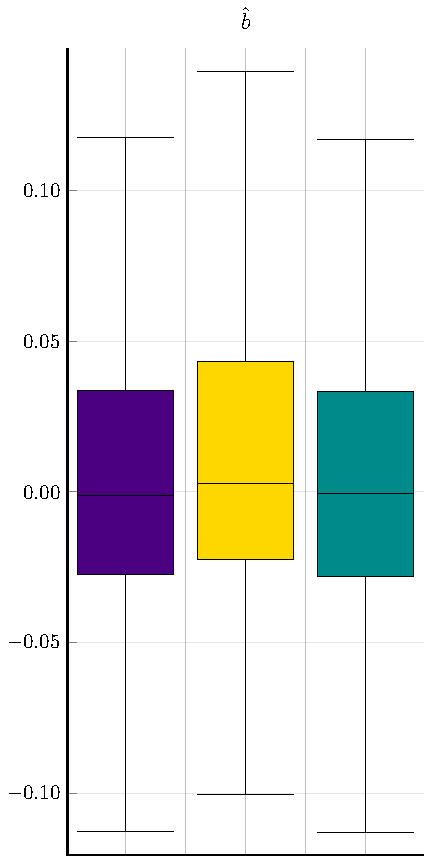
\includegraphics[width=.3\textwidth]{Figures/3/BIAS_b.pdf} & 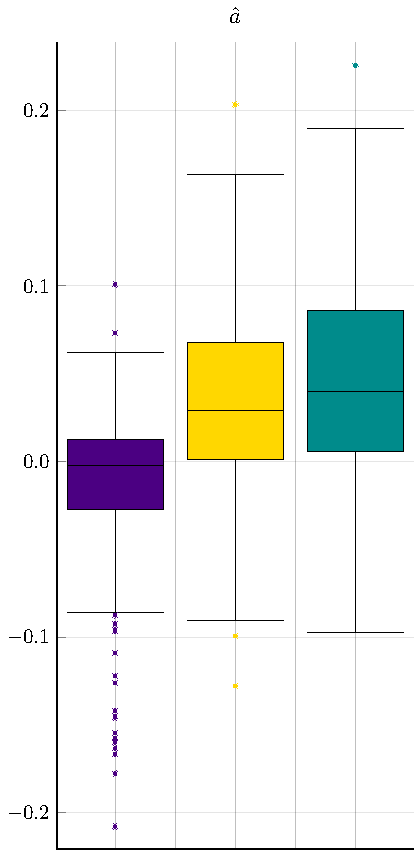
\includegraphics[width=.3\textwidth]{Figures/3/BIAS_a.pdf} & 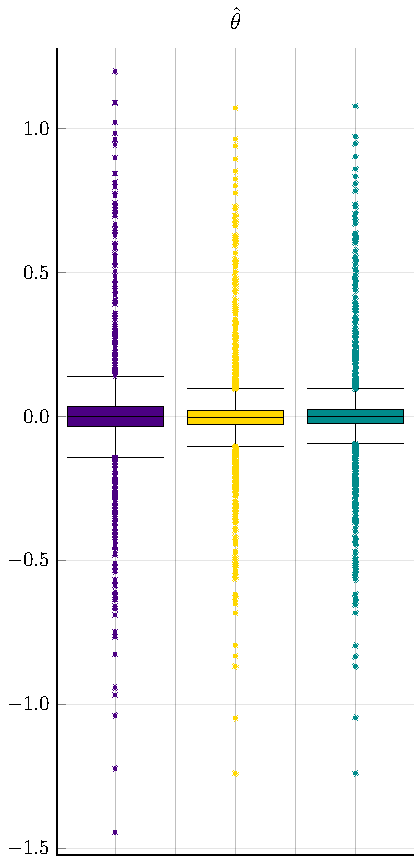
\includegraphics[width=.3\textwidth]{Figures/3/BIAS_t.pdf}
	\end{tabular}
	\caption{Case 3 - Boxplots of BIASs.}
	\label{fig:bpBIAS3}
\end{figure}
\begin{figure}[H] 
	\centering
	%\textbf{RMSEs of estimates with respect to the true values of item parameters and ability }\par\medskip
	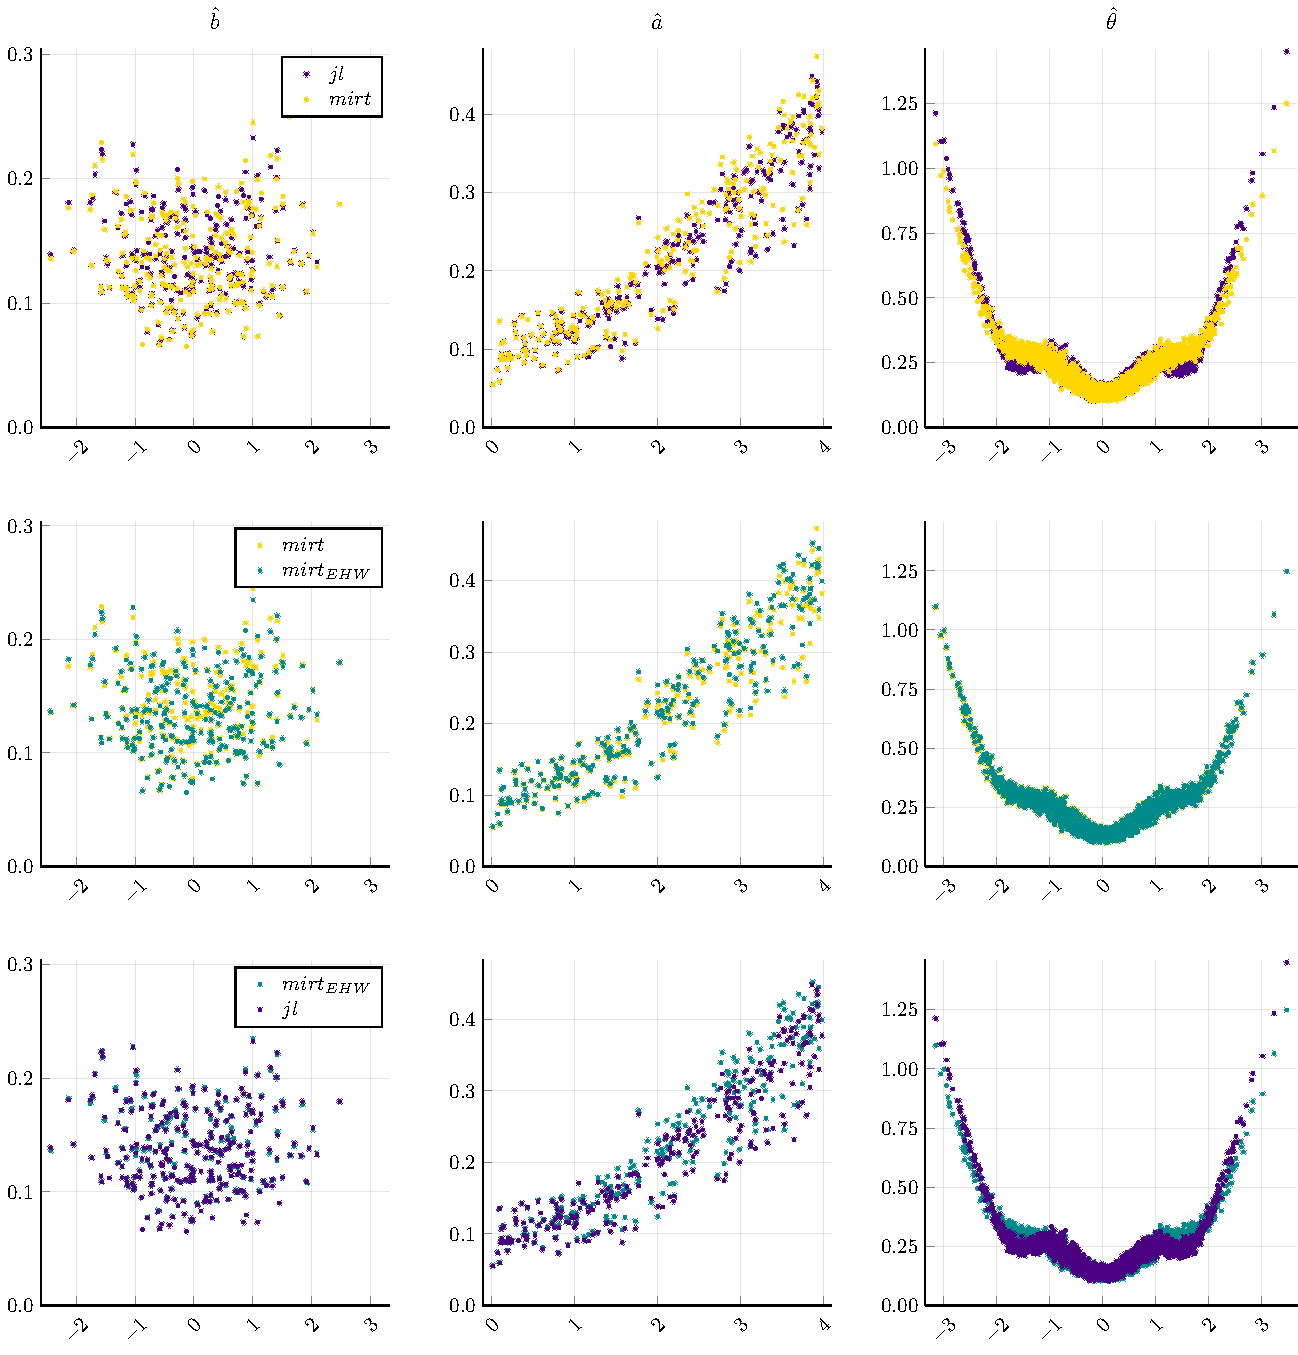
\includegraphics[width=\textwidth]{Figures/3/RMSEscatter.pdf}
	\caption{Case 3 - Scatter plots of RMSEs.}
	\label{fig:spRMSE3}
\end{figure}
\begin{figure}[H] 
	\centering
	%\textbf{BIASs of estimates with respect to the true values of item parameters and ability}\par\medskip
	\includegraphics[width=\textwidth]{Figures/3/BIASscatter.pdf}
	\caption{Case 3 - Scatter plots of BIASs }
	\label{fig:spBIAS3}
\end{figure}
\subsection{Case 4}
\begin{figure}[H] 
	\centering
	\begin{tabular}[b]{c c c}
		\includegraphics[width=.3\textwidth]{Figures/4/RMSE_b.pdf} & \includegraphics[width=.3\textwidth]{Figures/4/RMSE_a.pdf} & \includegraphics[width=.3\textwidth]{Figures/4/RMSE_t.pdf}
	\end{tabular}
	\caption{Case 4 - Boxplots of RMSEs.}
	\label{fig:bpRMSE4}
\end{figure}
\begin{figure}[H] 
	
	\centering
	\begin{tabular}[b]{c c c}
		\includegraphics[width=.3\textwidth]{Figures/4/BIAS_b.pdf} & \includegraphics[width=.3\textwidth]{Figures/4/BIAS_a.pdf} & \includegraphics[width=.3\textwidth]{Figures/4/BIAS_t.pdf}
	\end{tabular}
	\caption{Case 4 - Boxplots of BIASs.}
	\label{fig:bpBIAS4}
\end{figure}
\begin{figure}[H] 
	\centering
	%\textbf{RMSEs of estimates with respect to the true values of item parameters and ability }\par\medskip
	\includegraphics[width=\textwidth]{Figures/4/RMSEscatter.pdf}
	\caption{Case 4 - Scatter plots of RMSEs.}
	\label{fig:spRMSE4}
\end{figure}
\begin{figure}[H] 
	\centering
	%\textbf{BIASs of estimates with respect to the true values of item parameters and ability}\par\medskip
	\includegraphics[width=\textwidth]{Figures/4/BIASscatter.pdf}
	\caption{Case 4 - Scatter plots of BIASs }
	\label{fig:spBIAS4}
\end{figure}

\section{Chance-constrained test assembly}

\subsection{Application on real data}

\begin{table}[H] 
	\centering
	\caption{Structure of assembled tests. }
	\label{tab:tast}
	\scriptsize
	\texttt{
		\begin{tabular}{cccc}
			\toprule
			test & length & DOMAIN\footnote{The order is: \{numbers; space and figures; data and forecasting; functions and relationships\}.} & overlap\footnote{From test 1 to test 20.} \\
			\midrule
			1 & 46 &\{ 12;12;12;10 \} & \{46;10;10;11;11;10;11;10;11;11;10;10;08;11;10;11;11;10;11;11\}
			\\
			2 & 45& \{ 12;12;12;09 \}& \{10;45;11;11;10;11;10;11;11;11;11;11;10;11;10;11;11;11;11;11\}
			\\
			3 & 45& \{ 11;12;12;09 \}& \{10;11;45;11;11;10;11;11;11;11;11;10;10;11;10;10;09;11;10;11\}
			\\
			4 & 45& \{ 12;12;12;09 \}& \{11;11;11;45;11;11;11;11;10;09;11;11;11;11;11;11;10;09;11;08\}
			\\
			5 & 44& \{ 12;12;12;08 \}& \{11;10;11;11;44;11;10;11;10;11;10;09;10;11;11;11;11;10;11;11\}
			\\
			6 & 43& \{ 12;12;12;07 \}& \{10;11;10;11;11;43;11;11;11;10;08;11;11;11;11;11;10;11;10;10\}
			\\
			7 & 45& \{ 12;12;12;09 \}& \{11;10;11;11;10;11;45;10;11;11;11;11;08;11;11;11;10;11;11;11\}
			\\
			8 & 44& \{ 12;12;12;08 \}& \{10;11;11;11;11;11;10;44;11;11;09;11;11;09;09;11;11;11;10;11\}
			\\
			9 &46 & \{ 12;11;10;13 \}& \{11;11;11;10;10;11;11;11;46;10;11;10;11;11;10;10;11;09;11;11\}
			\\
			10 & 45& \{ 12;11;12;10 \}& \{11;11;11;09;11;10;11;11;10;45;11;11;11;09;11;10;09;11;11;10\}
			\\
			11 &44 & \{ 12;12;12;08 \}&\{10;11;11;11;10;08;11;09;11;11;44;10;10;10;07;08;11;11;08;11\}
			\\
			12 &45 & \{ 12;12;12;09 \}& \{10;11;10;11;09;11;11;11;10;11;10;45;11;11;11;11;11;11;10;09\}
			\\
			13 &45 & \{ 12;11;11;11 \}& \{08;10;10;11;10;11;08;11;11;11;10;11;45;11;09;11;10;11;11;11\}
			\\
			14 &45 & \{ 12;12;12;09 \}& \{11;11;11;11;11;11;11;09;11;09;10;11;11;45;08;11;11;08;10;10\}
			\\
			15 &45 & \{ 12;12;12;10 \}& \{10;10;10;11;11;11;11;09;10;11;07;11;09;08;46;11;11;09;11;11\}
			\\
			16 &46 & \{ 12;12;12;09 \}& \{11;11;10;11;11;11;11;11;10;10;08;11;11;11;11;45;11;11;11;05\}
			\\
			17 &45 & \{ 12;12;12;09 \}& \{11;11;09;10;11;10;10;11;11;09;11;11;10;11;11;11;45;11;09;11\}
			\\
			18 &45 & \{ 12;12;12;09 \}& \{10;11;11;09;10;11;11;11;09;11;11;11;11;08;09;11;11;45;11;11\}
			\\
			19 &45 & \{ 12;12;12;09 \}& \{11;11;10;11;11;10;11;10;11;11;08;10;11;10;11;11;09;11;45;10\}
			\\
			20 &45 & \{ 12;12;12;09 \}& \{11;11;11;08;11;10;11;11;11;10;11;09;11;10;11;05;11;11;10;45\}
			\\
			\bottomrule
	\end{tabular}}
\end{table}

\begin{figure}[H]
	
	\centering
	\begin{subfigure}[t]{0.31\textwidth}	
		\centering
		\includegraphics[width=\linewidth]{Figures/real/1_infoplot.pdf}
		\caption{t=1} 
	\end{subfigure}
	\begin{subfigure}[t]{0.31\textwidth}
		\centering
		\includegraphics[width=\linewidth]{Figures/real/2_infoplot.pdf}
		\caption{t=2} 
	\end{subfigure}\\
	\begin{subfigure}[t]{0.31\textwidth}
		\centering
		\includegraphics[width=\linewidth]{Figures/real/3_infoplot.pdf}
		\caption{t=3} 
	\end{subfigure}
	\begin{subfigure}[t]{0.31\textwidth}
		\centering
		\includegraphics[width=\linewidth]{Figures/real/4_infoplot.pdf}
		\caption{t=4} 
	\end{subfigure}\\
	\begin{subfigure}[t]{0.31\textwidth}
		\centering
		\includegraphics[width=\linewidth]{Figures/real/5_infoplot.pdf}
		\caption{t=5} 
	\end{subfigure}
	\begin{subfigure}[t]{0.31\textwidth}
		\centering
		\includegraphics[width=\linewidth]{Figures/real/6_infoplot.pdf}
		\caption{t=6} 
	\end{subfigure}\\
	\begin{subfigure}[t]{0.31\textwidth}
		\centering
		\includegraphics[width=\linewidth]{Figures/real/7_infoplot.pdf}
		\caption{t=7} 
	\end{subfigure}
	\begin{subfigure}[t]{0.31\textwidth}
		\centering
		\includegraphics[width=\linewidth]{Figures/real/8_infoplot.pdf}
		\caption{t=8} 
	\end{subfigure}\\
	\begin{subfigure}[t]{0.31\textwidth}
		\centering
		\includegraphics[width=\linewidth]{Figures/real/9_infoplot.pdf}
		\caption{t=9} 
	\end{subfigure}
	\begin{subfigure}[t]{0.31\textwidth}
		\centering
		\includegraphics[width=\linewidth]{Figures/real/10_infoplot.pdf}
		\caption{t=10} 
	\end{subfigure}
	\caption{Sampling distributions of TIFs. Tests 1-10. The horizontal axis represents the latent trait $\theta$	\label{fig:taTIF}}
\end{figure}

\begin{figure}[H]
	
	\centering
	\begin{subfigure}[t]{0.31\textwidth}	
		\centering
		\includegraphics[width=\linewidth]{Figures/real/11_infoplot.pdf}
		\caption{t=11} 
	\end{subfigure}
	\begin{subfigure}[t]{0.31\textwidth}
		\centering
		\includegraphics[width=\linewidth]{Figures/real/12_infoplot.pdf}
		\caption{t=12} 
	\end{subfigure}\\
	\begin{subfigure}[t]{0.31\textwidth}
		\centering
		\includegraphics[width=\linewidth]{Figures/real/13_infoplot.pdf}
		\caption{t=13} 
	\end{subfigure}
	\begin{subfigure}[t]{0.31\textwidth}
		\centering
		\includegraphics[width=\linewidth]{Figures/real/14_infoplot.pdf}
		\caption{t=14} 
	\end{subfigure}\\
	\begin{subfigure}[t]{0.31\textwidth}
		\centering
		\includegraphics[width=\linewidth]{Figures/real/15_infoplot.pdf}
		\caption{t=15} 
	\end{subfigure}
	\begin{subfigure}[t]{0.31\textwidth}
		\centering
		\includegraphics[width=\linewidth]{Figures/real/16_infoplot.pdf}
		\caption{t=16} 
	\end{subfigure}\\
	\begin{subfigure}[t]{0.31\textwidth}
		\centering
		\includegraphics[width=\linewidth]{Figures/real/17_infoplot.pdf}
		\caption{t=17} 
	\end{subfigure}
	\begin{subfigure}[t]{0.31\textwidth}
		\centering
		\includegraphics[width=\linewidth]{Figures/real/18_infoplot.pdf}
		\caption{t=18} 
	\end{subfigure}\\
	\begin{subfigure}[t]{0.31\textwidth}
		\centering
		\includegraphics[width=\linewidth]{Figures/real/19_infoplot.pdf}
		\caption{t=19} 
	\end{subfigure}
	\begin{subfigure}[t]{0.31\textwidth}
		\centering
		\includegraphics[width=\linewidth]{Figures/real/20_infoplot.pdf}
		\caption{t=20} 
	\end{subfigure}
	\caption{Sampling distributions of TIFs. Tests 11-20. The horizontal axis represents the latent trait $\theta$. \label{fig:taTIF2}}
\end{figure}

\begin{figure}[H]
	
	\centering
	\begin{subfigure}[t]{0.8\textwidth}	
		\centering
		\includegraphics[width=\linewidth]{Figures/real/TIFPlot.pdf}
		\caption{TIF}
	\end{subfigure}\\
	\begin{subfigure}[t]{0.8\textwidth}
		\centering
		\includegraphics[width=\linewidth]{Figures/real/ICFPlot.pdf}
		\caption{ICC}
	\end{subfigure}
	\caption{TIFs and Item characteristic curves (ICCs) obtained from the full sample. The horizontal axis represents the latent trait $\theta$. \label{fig:taTIFICF}}
\end{figure}
